\subsection{Obtaining conformal confidence sets with increasing combination functions}\label{A:CF}
As discussed in Remark \ref{rmk:max} the results of Sections \ref{SS:MCS} and \ref{SS:joint} can be generalized to a wider class of combination functions. 
\begin{definition}
	We define a suitable combination function to be a function $C: \mathcal{P}(\mathcal{V}) \times \mathcal{X} \rightarrow \mathbb{R}$  which is increasing in the sense that for all sets $\mathcal{A} \subseteq \mathcal{V}$ and each $v \in \mathcal{A} $, $C(v, X) \leq C(\mathcal{A}, X)$ for all $X \in \mathcal{X}$. 
\end{definition}
The maximum is a suitable combination function since $X(v) = \max_{v \in \lbrace v \rbrace } X(v) \leq \max_{v \in \mathcal{A}} X(v)$. As such this framework directly generalizes the results of the main text. 
%Moreover for each $1\leq i \leq n + 1$, let $$\tau'_i = C(\lbrace v \in \mathcal{V}: Y_i(v) = 0\rbrace, f_O(s(X_i))) $$and $$\gamma'_i= C(\lbrace v \in \mathcal{V}: Y_i(v) = 1\rbrace, f_I(-s(X_i))).$$

We can construct generalized marginal confidence sets as follows.
\begin{theorem}
	(Marginal inner set)
	Under Assumptions \ref{ass:ex} and \ref{ass:indep}, given $\alpha_1 \in (0,1)$, let 
	\begin{equation*}
		\lambda_I(\alpha_1) = \inf\left\lbrace \lambda: \frac{1}{n} \sum_{i = 1}^n 1\left[ C(\lbrace v \in \mathcal{V}: Y_i(v) = 1\rbrace, f_I(-s(X_i))) \leq \lambda \right] \geq \alpha_1 \right\rbrace,
	\end{equation*}
 	for a suitable combination function $C$, and define $I(X) = \lbrace v \in \mathcal{V}: C(v, f_I(-s(X))) >\lambda_I(\alpha_1)  \rbrace $. Then,
	\begin{equation}\label{eq:probstat}
		\mathbb{P}\left( I(X) \subseteq\lbrace v\in \mathcal{V}: Y_{n+1} = 1 \rbrace \right) \geq 1 - \alpha_1.
	\end{equation}
\end{theorem}
The proof follows that of Theorem \ref{thm:inner}. The key observation is that for any suitable combination function $C$,  given $\lambda \in \mathbb{R}$, $\mathcal{A} \subseteq \mathcal{V} $ and $X \in \mathcal{X}$, we have that $C(\mathcal{A}, X) \leq \lambda$ implies that $C(v, X) \leq \lambda$. This is the relevant property of the maximum which we used for the results in the main text. For the outer set we similarly have the following.
\begin{theorem}
	(Marginal outer set)
	Under Assumptions \ref{ass:ex} and \ref{ass:indep}, given $\alpha_2 \in (0,1)$, let 
	\begin{equation*}
		\lambda_O({\alpha_2})= \inf\left\lbrace \lambda: \frac{1}{n} \sum_{i = 1}^n 1\left[ C(\lbrace v \in \mathcal{V}: Y_i(v) = 0\rbrace, f_O(s(X_i))) \leq \lambda \right] \geq \alpha_2 \right\rbrace.
	\end{equation*}
	for a suitable combination function $C$, and define $O(X) = \lbrace v \in \mathcal{V}: C(v, f_O(s(X))) >\lambda_O(\alpha_2)  \rbrace $. Then,
	\begin{equation}\label{eq:probstat}
		\mathbb{P}\left( \lbrace v\in \mathcal{V}: Y_{n+1}(v) = 1 \rbrace \subseteq O(X_{n+1}) \right) \geq 1 - \alpha_2.
	\end{equation}
\end{theorem}
Joint results can be analogously obtained. 

\newpage
\subsection{Additional examples from the learning dataset}

\begin{figure}[h!]
	%	\centering
	\begin{center}
		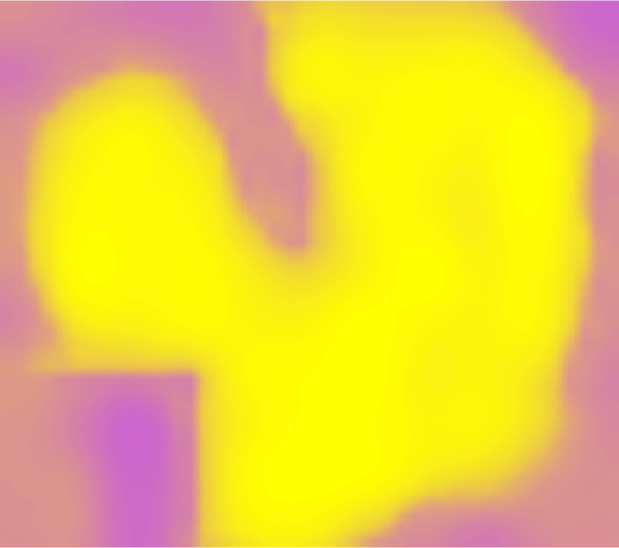
\includegraphics[width=0.24\textwidth]{../figures/learning/scores/772.png}
		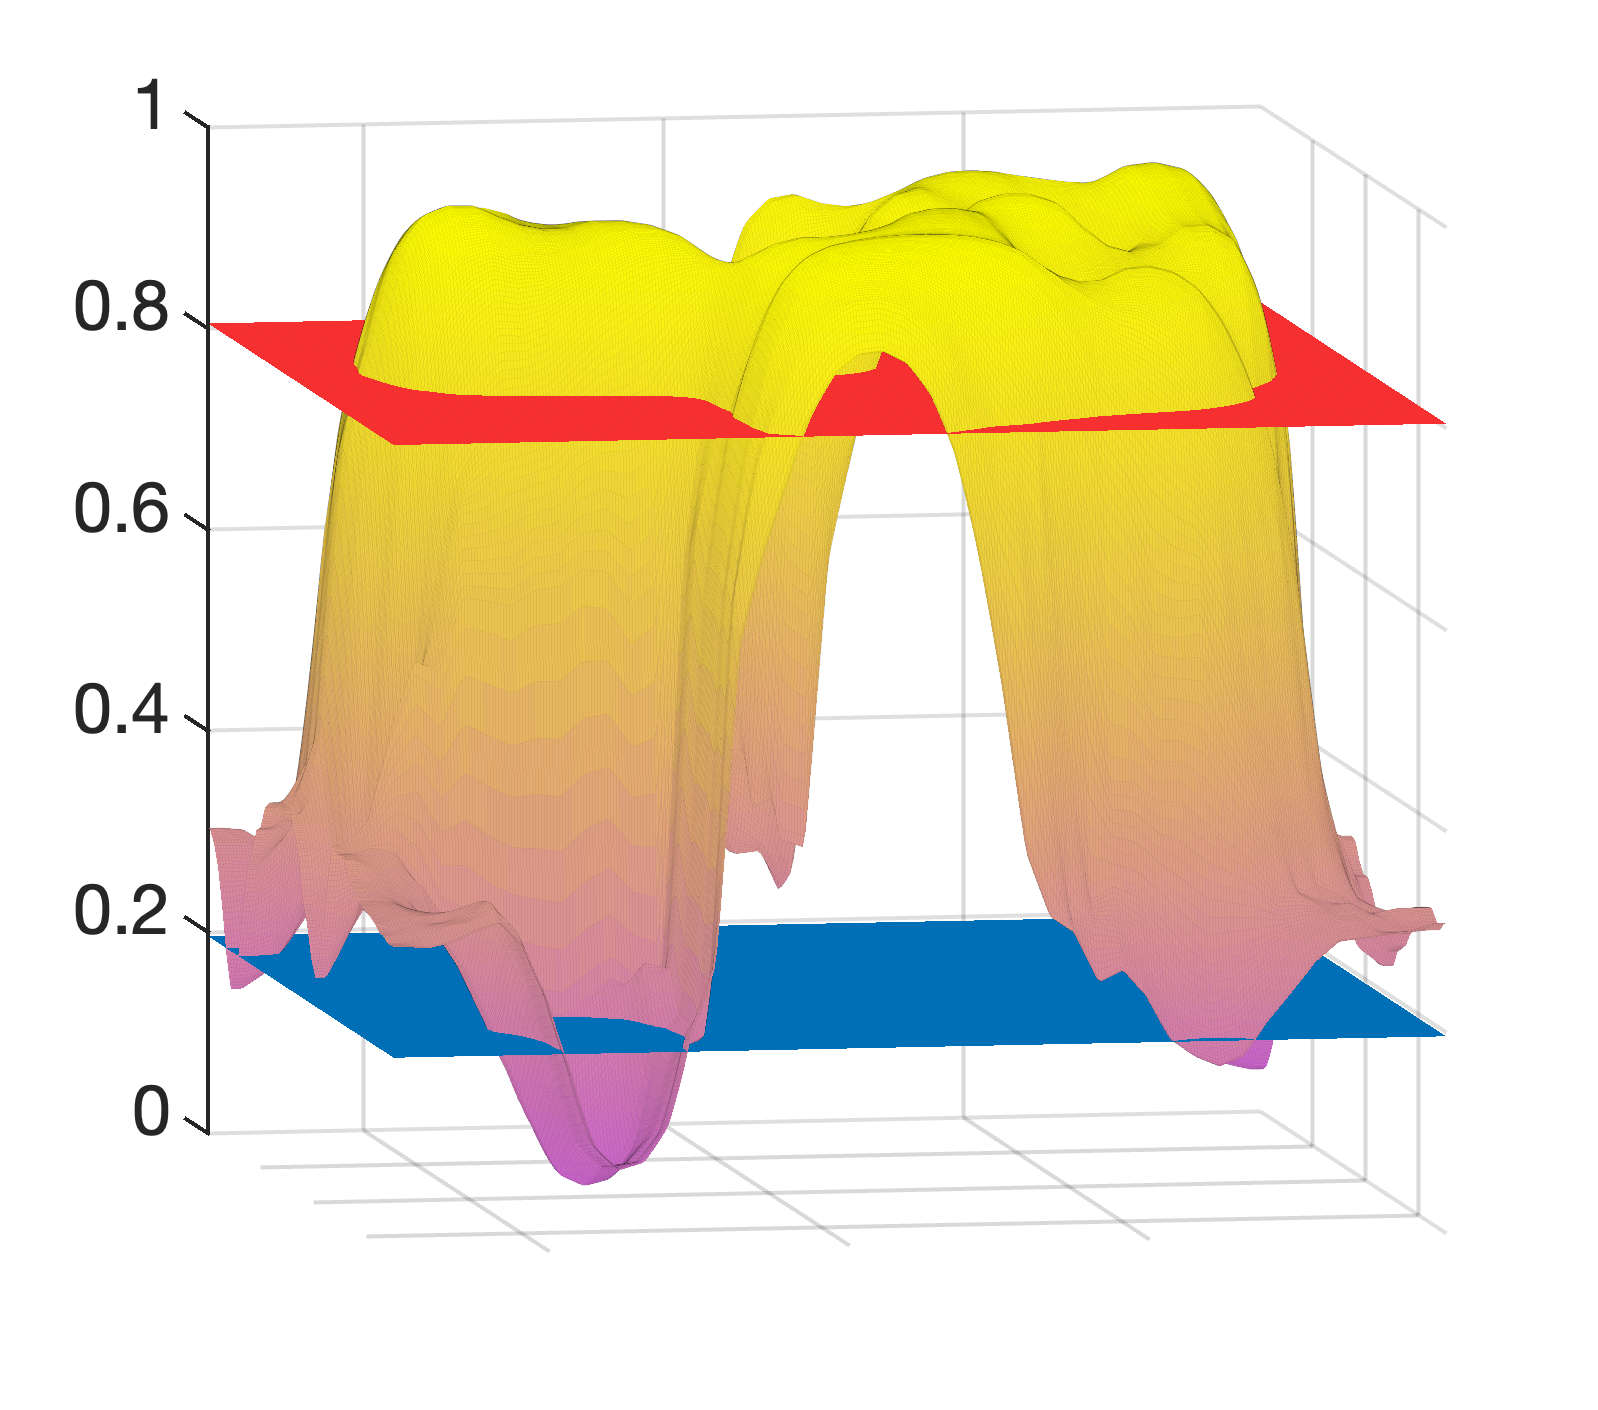
\includegraphics[width=0.24\textwidth]{../figures/learning/score_surf/772.png}	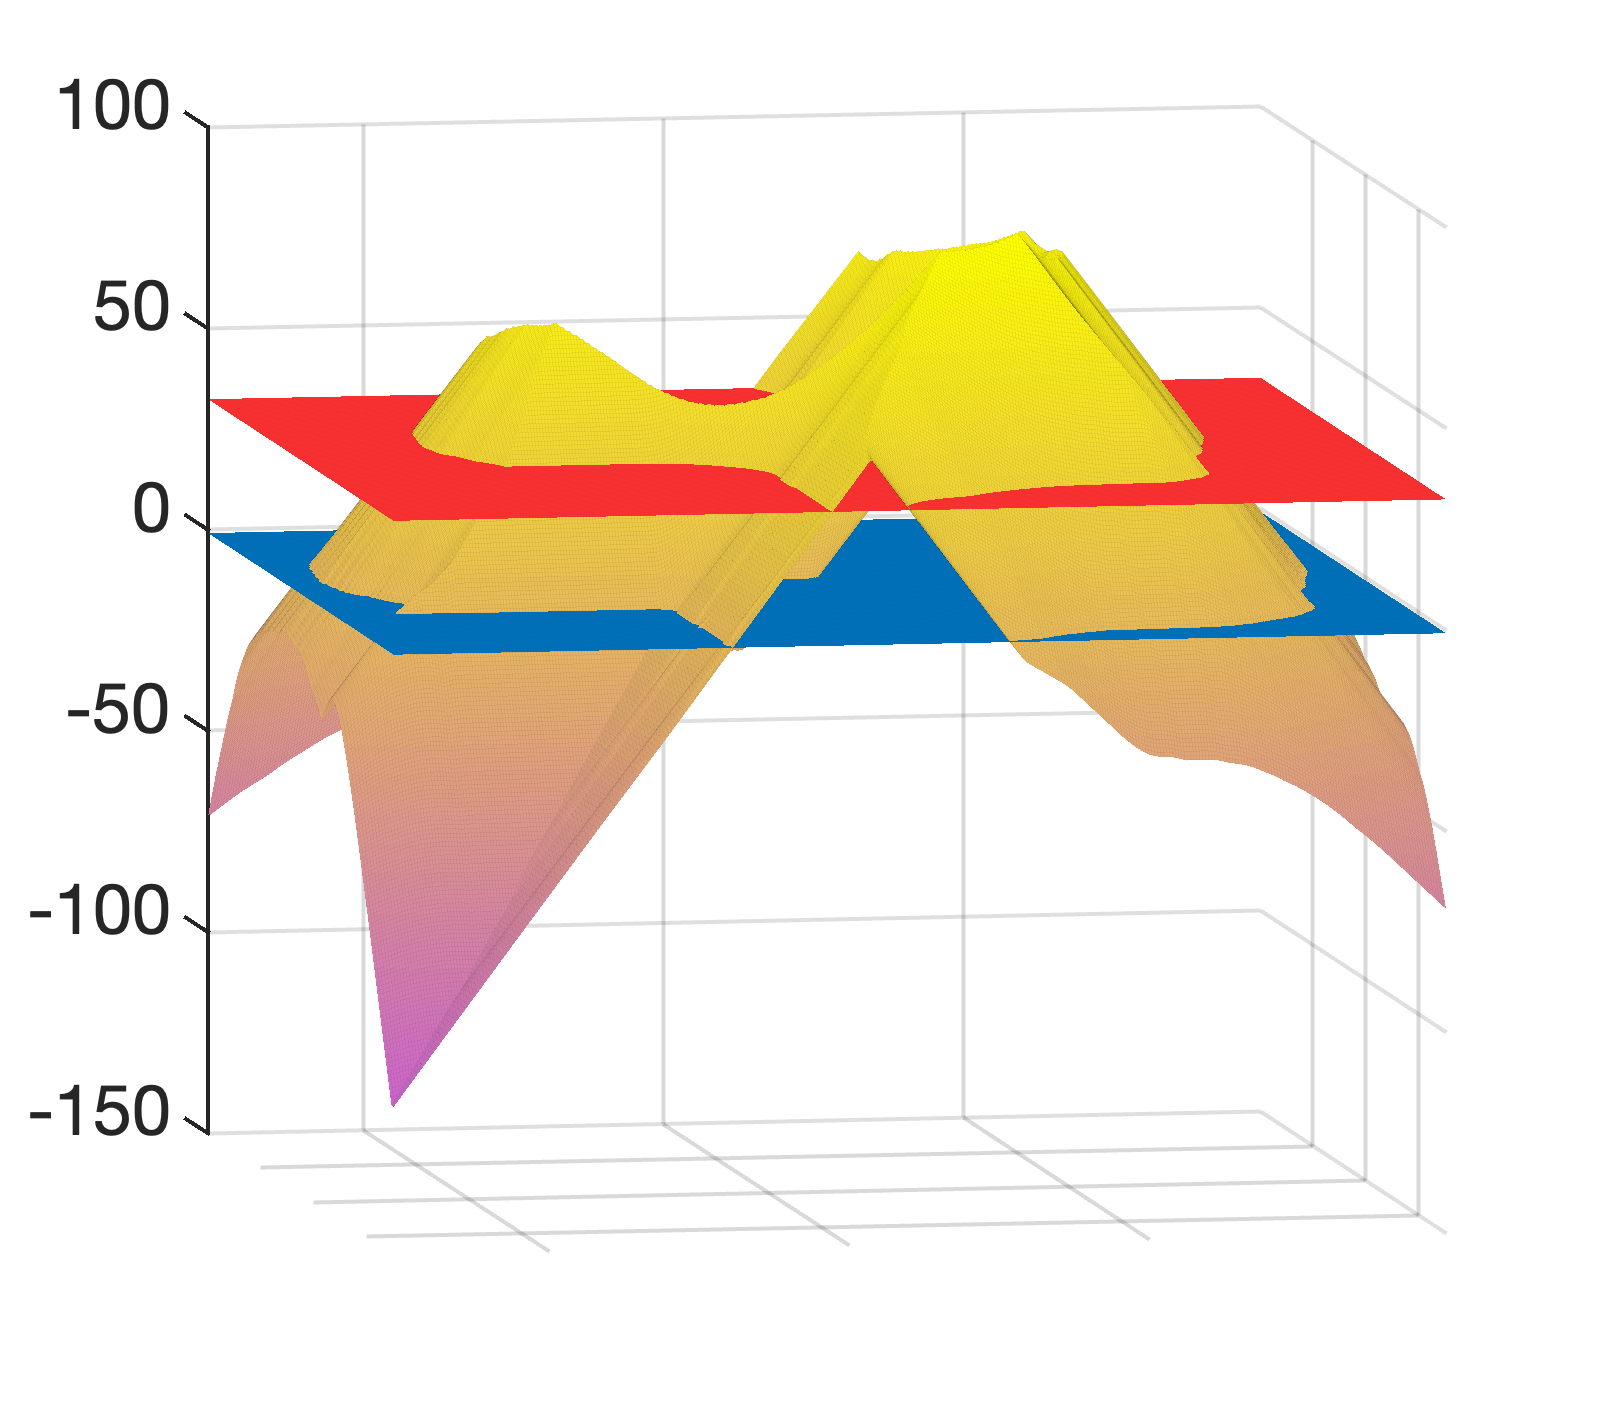
\includegraphics[width=0.24\textwidth]{../figures/learning/dist_surf/772.png}
		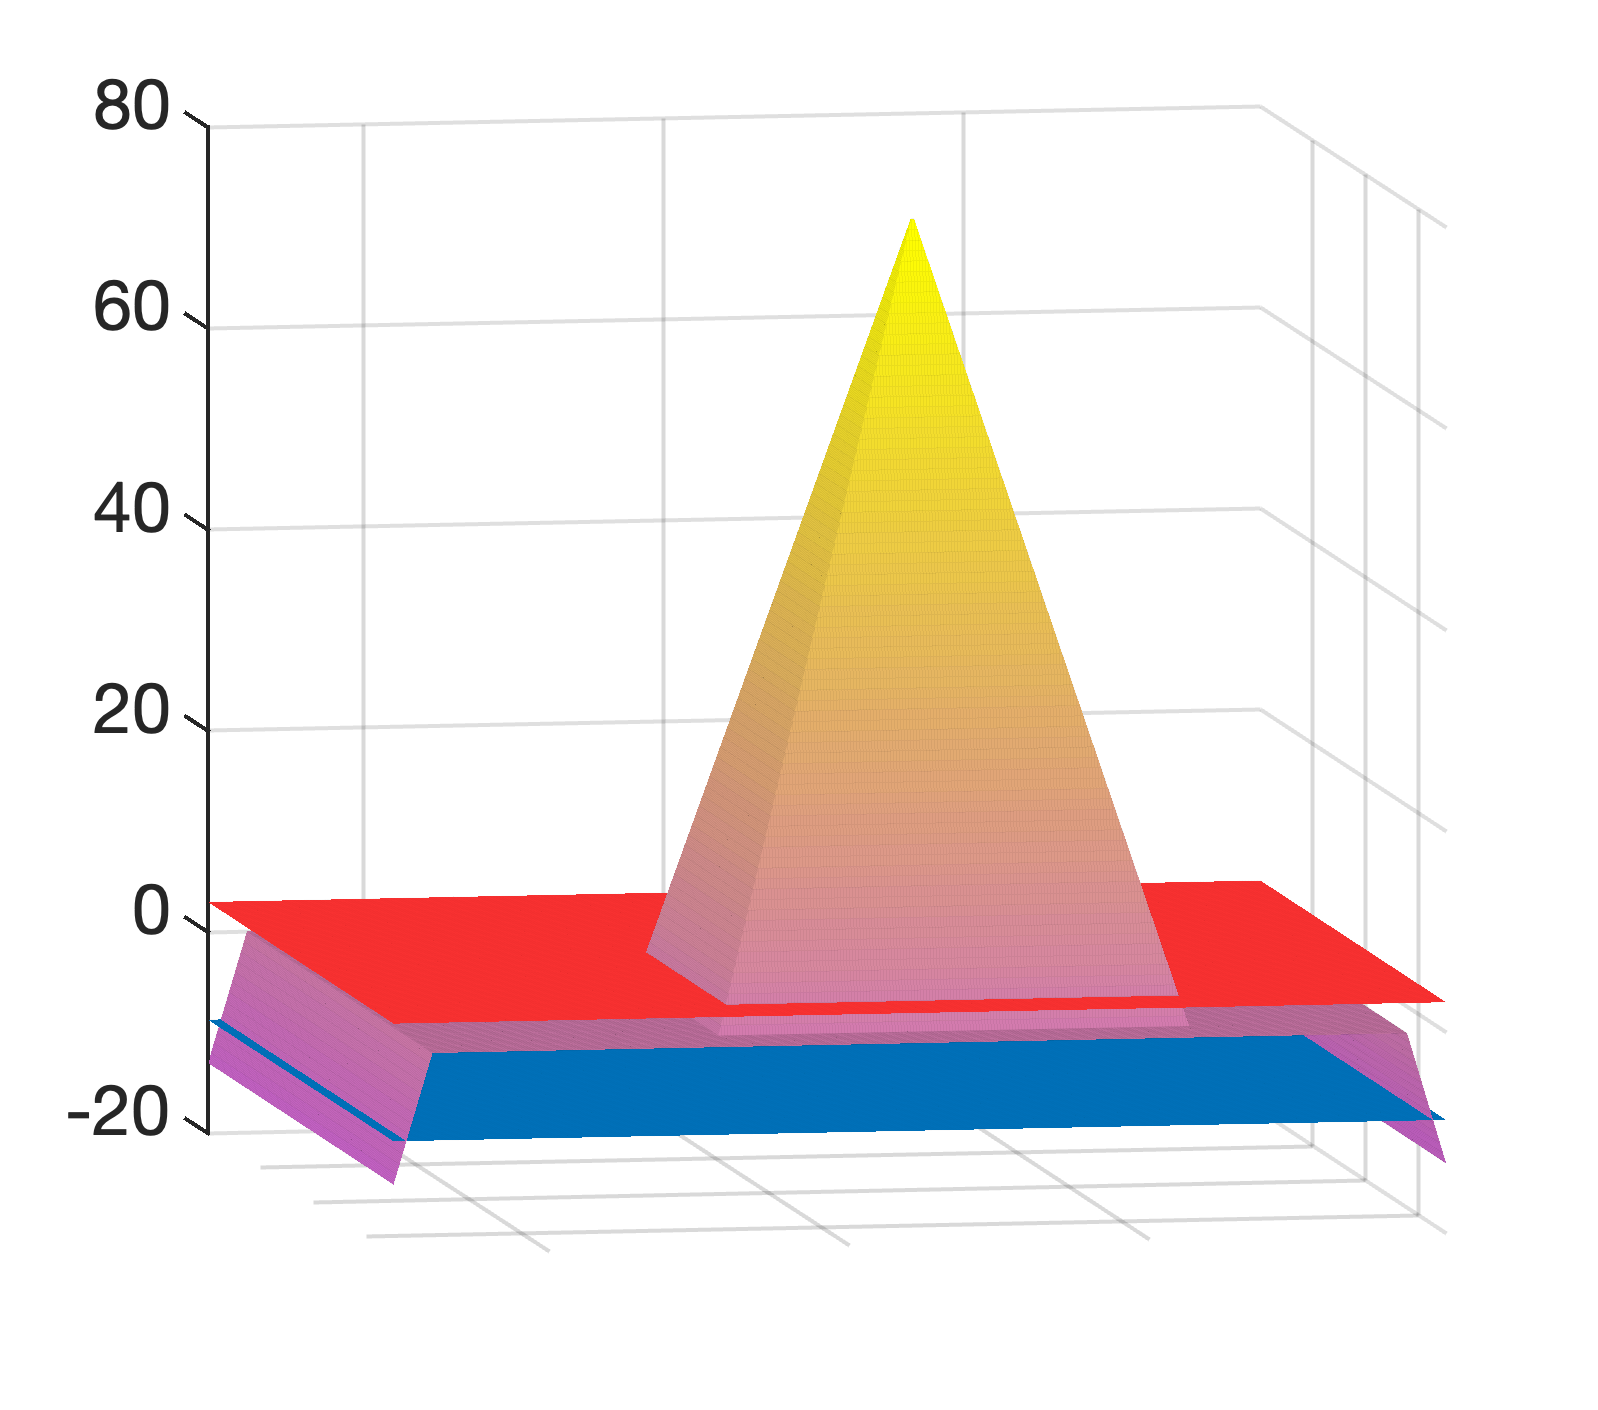
\includegraphics[width=0.24\textwidth]{../figures/learning/dist_bt_surf/772.png}\\
		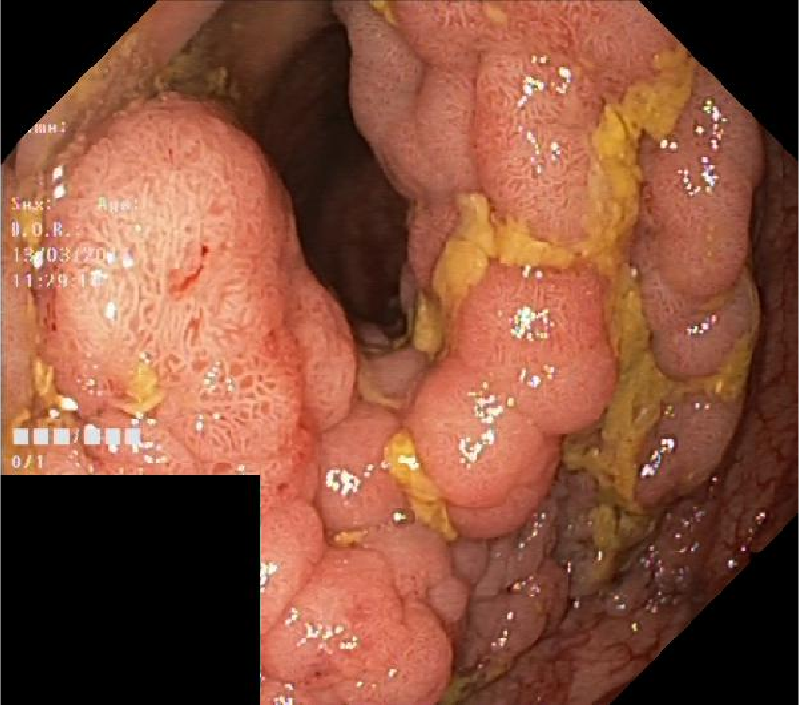
\includegraphics[width=0.24\textwidth]{../figures/learning/images/772.png}
		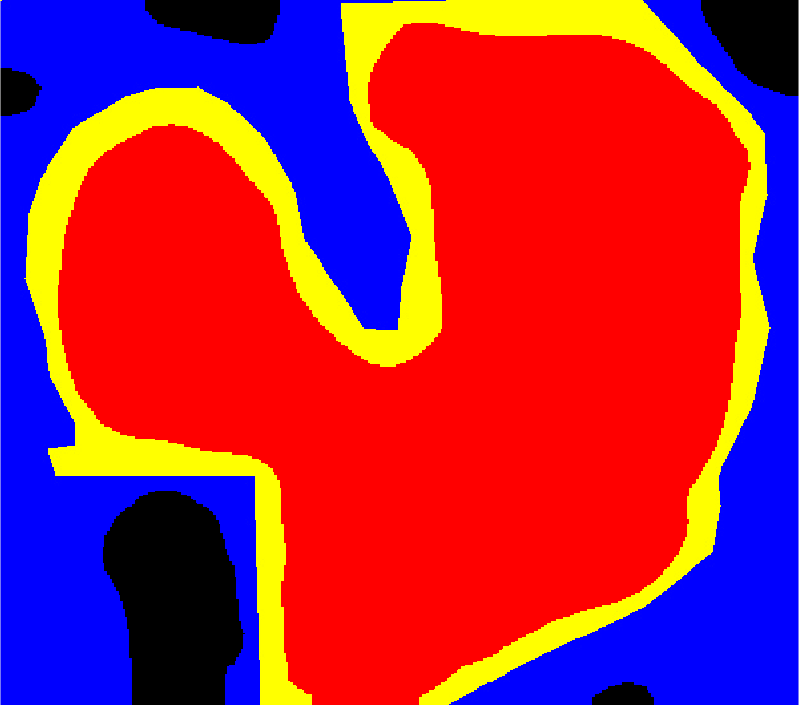
\includegraphics[width=0.24\textwidth]{../figures/learning/score_crs_marginal90/772.png}
		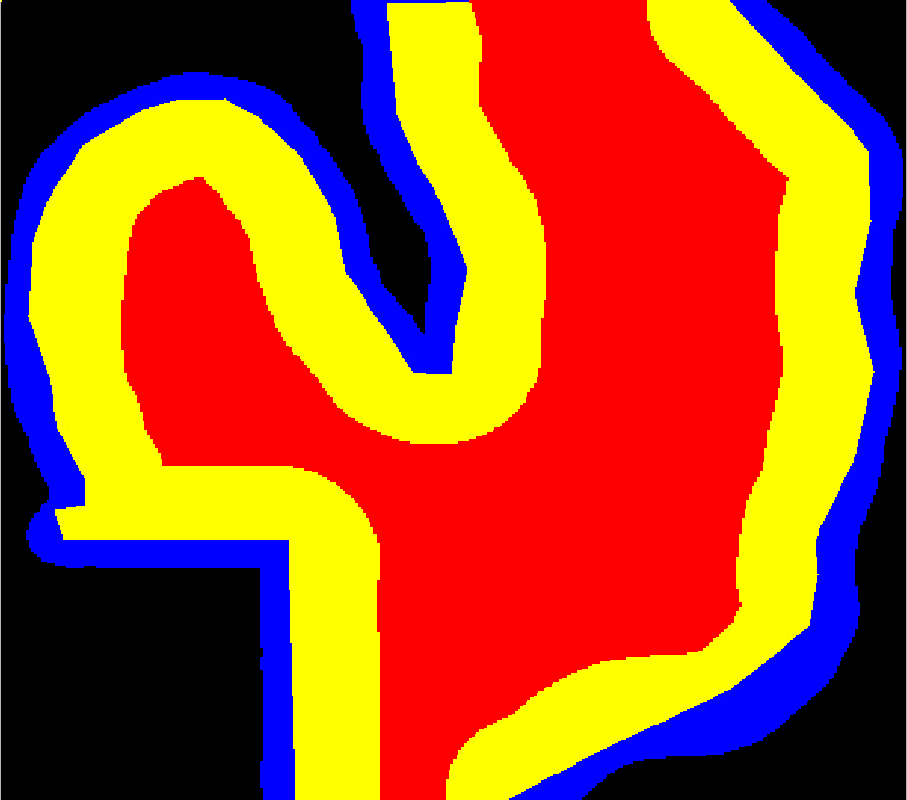
\includegraphics[width=0.24\textwidth]{../figures/learning/dist_crs_marginal90/772.png}
		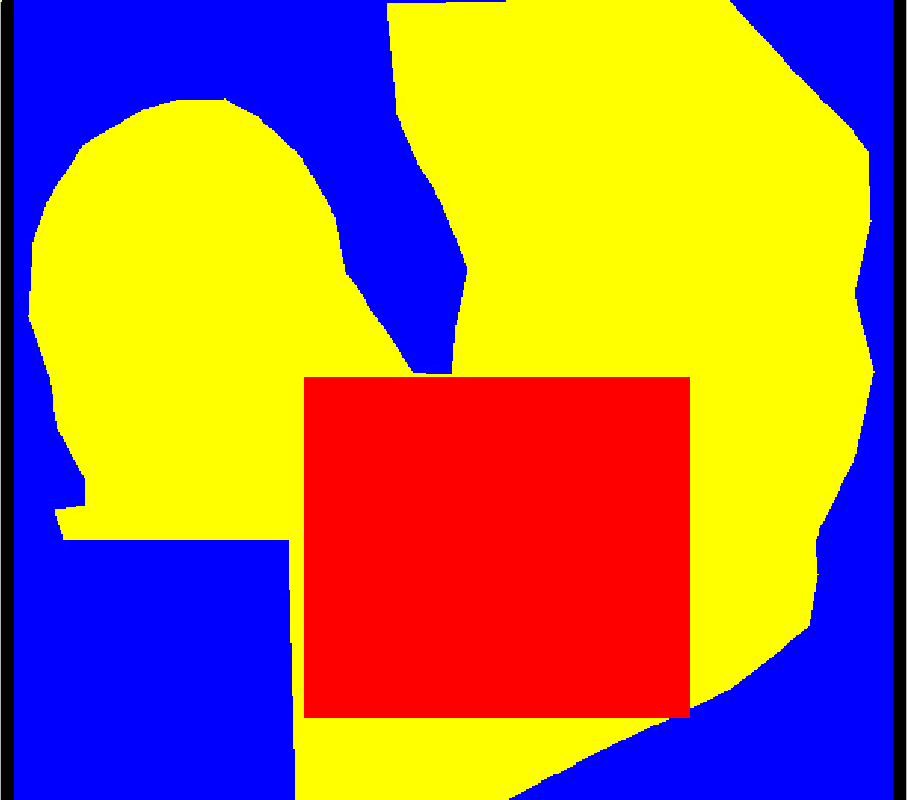
\includegraphics[width=0.24\textwidth]{../figures/learning/dist_bt_crs_marginal90/772.png}\\
		\vspace{0.5cm}
		
\includegraphics[width=0.24\textwidth]{../figures/learning/scores/903.png}
		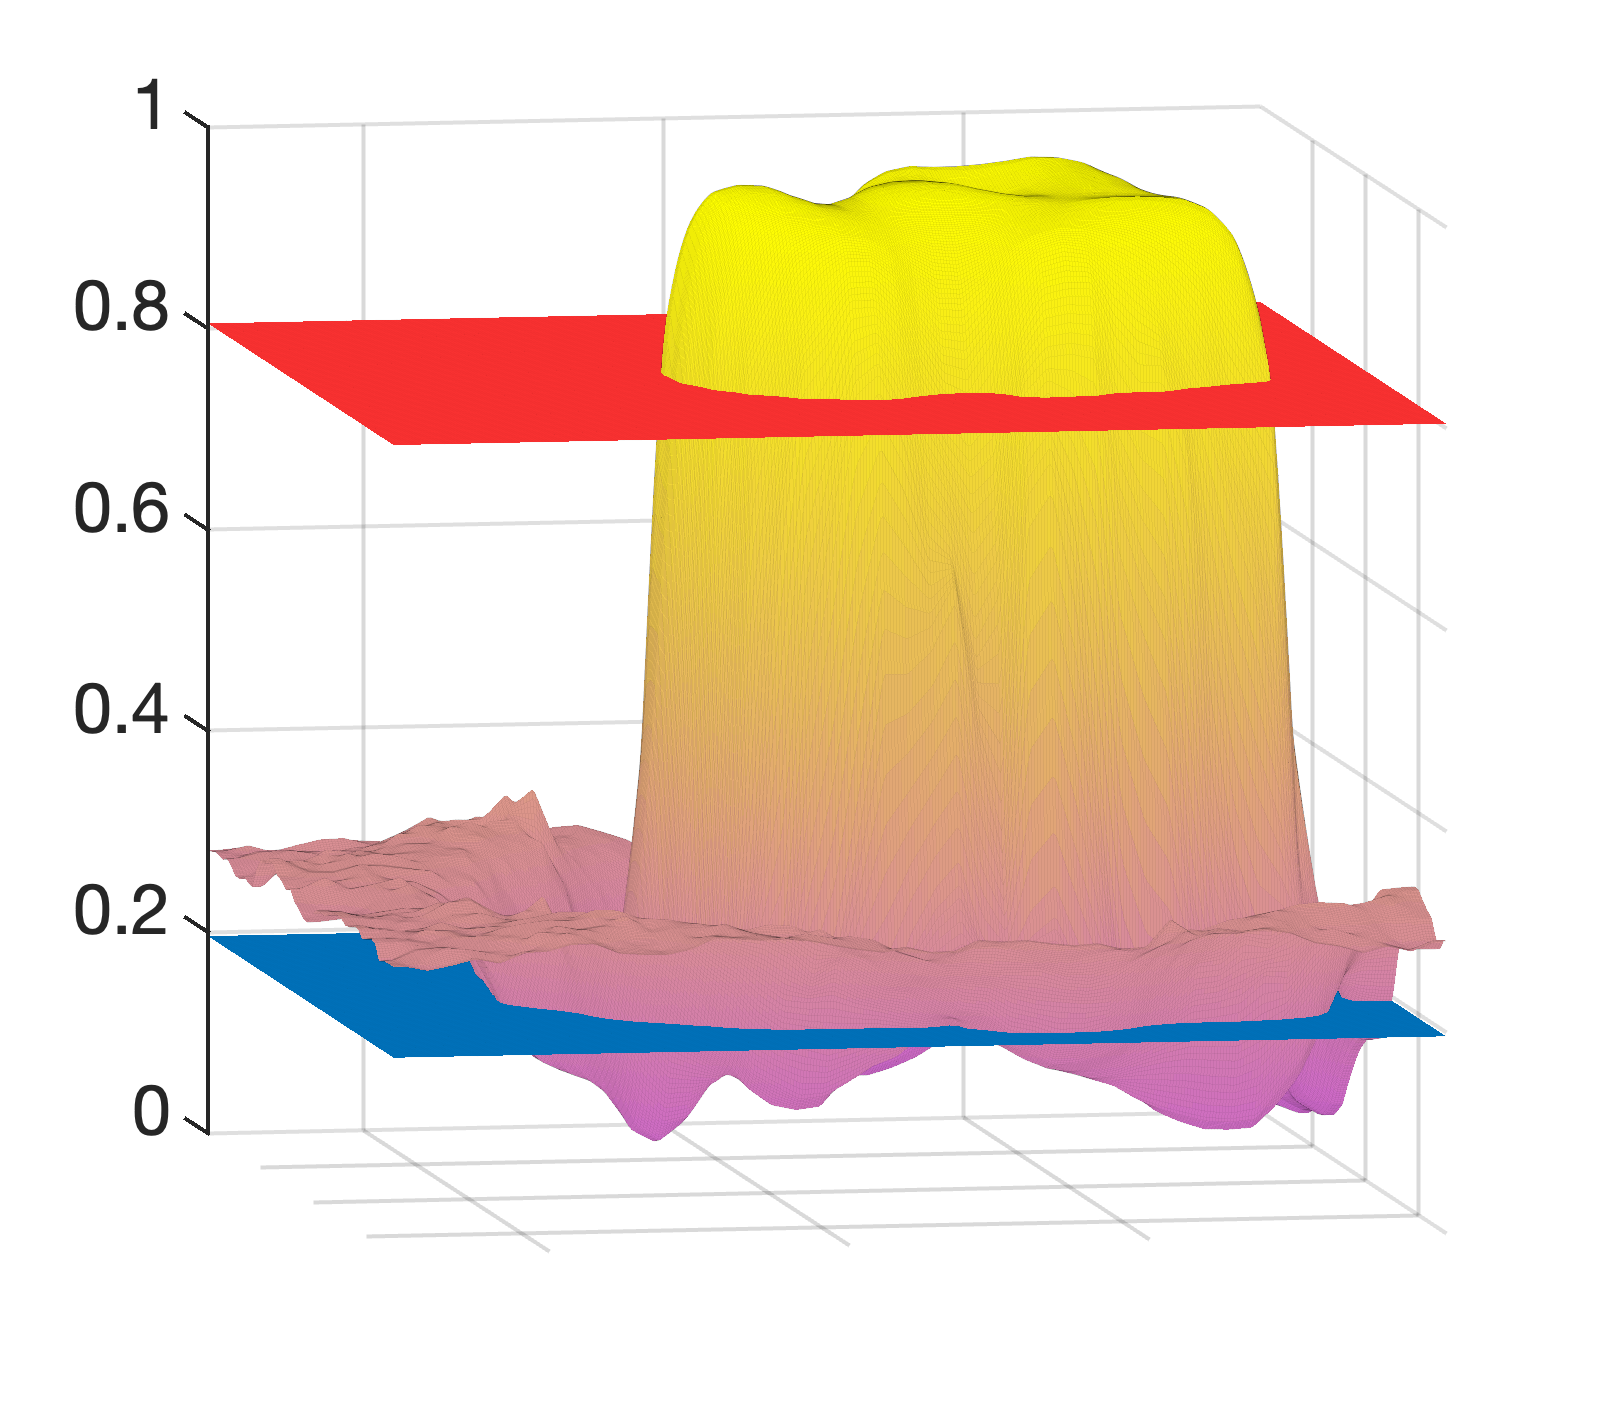
\includegraphics[width=0.24\textwidth]{../figures/learning/score_surf/903.png}	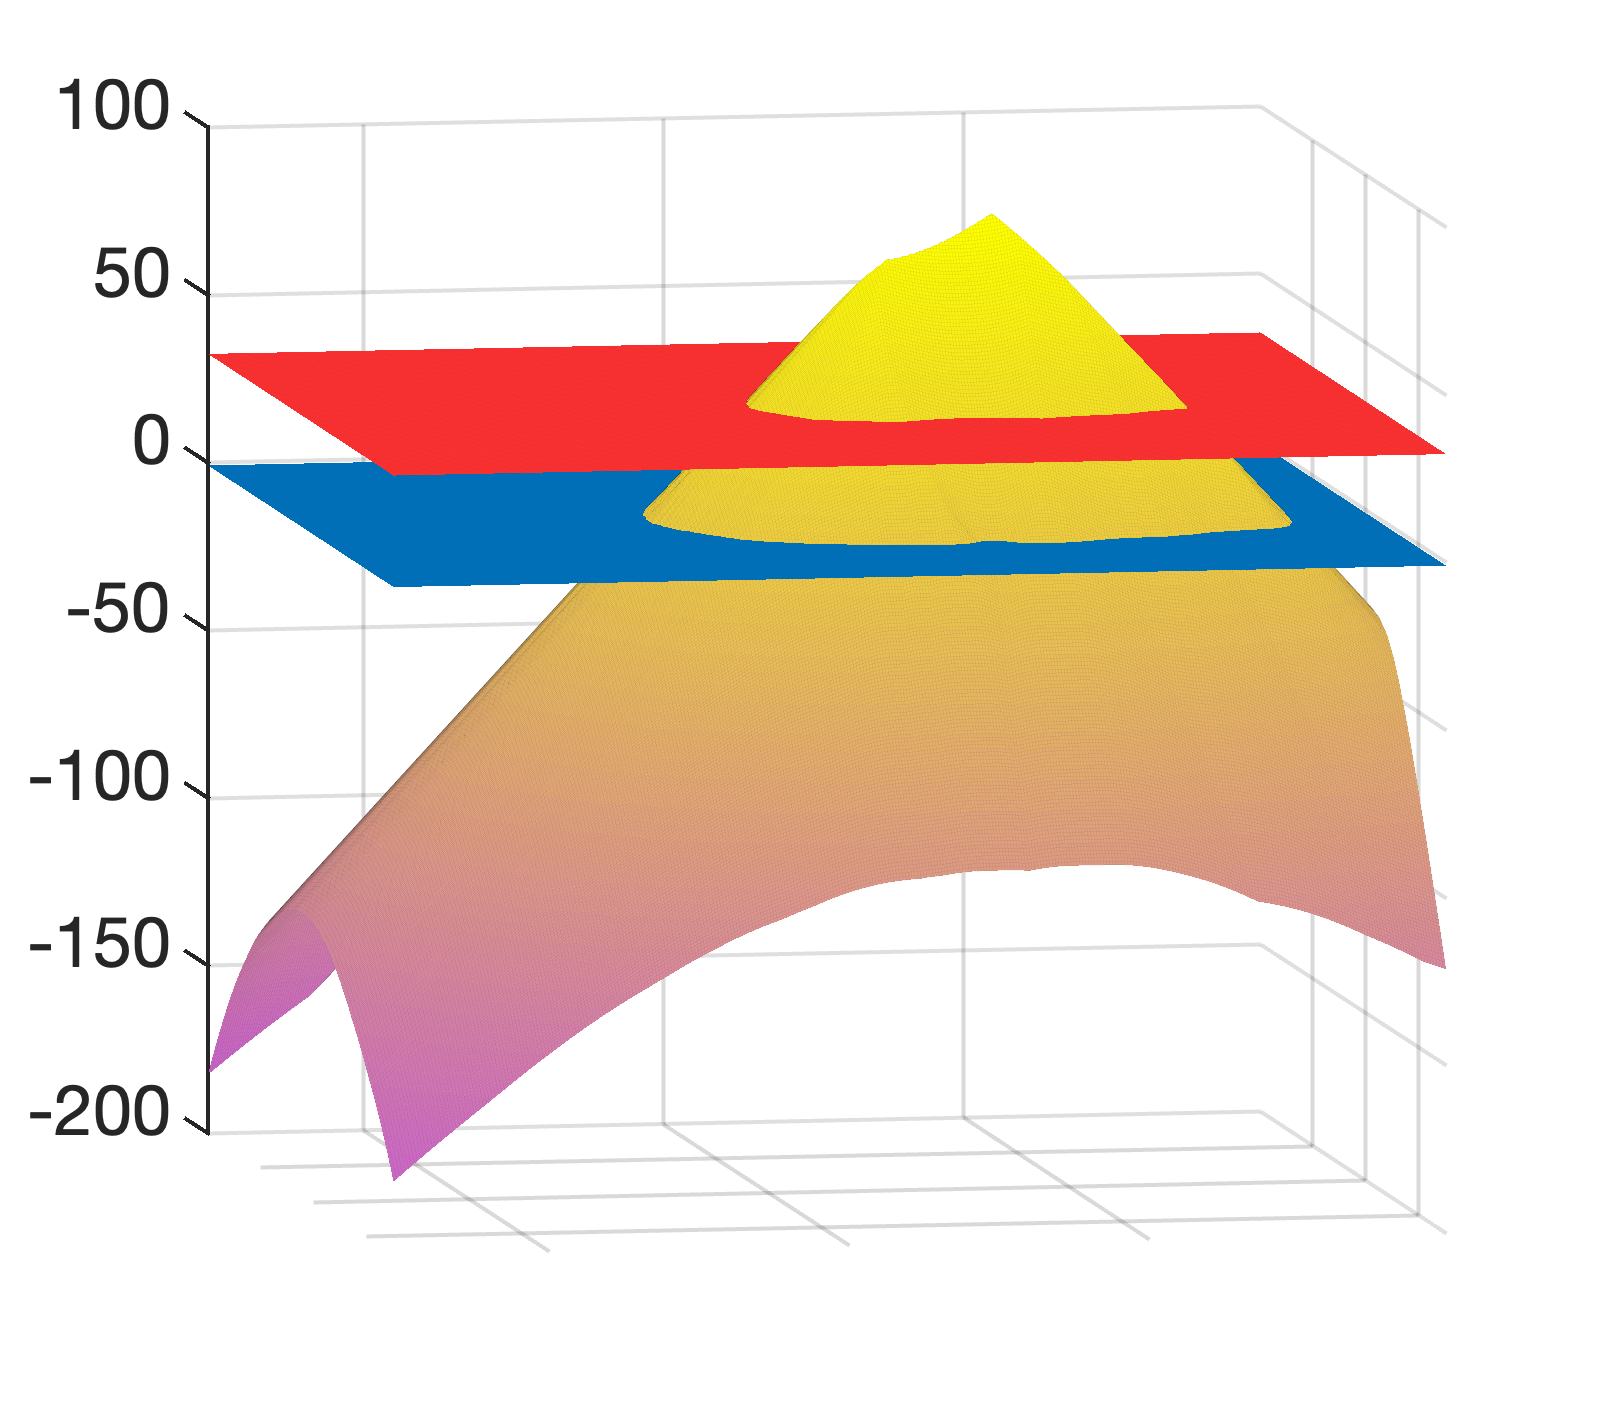
\includegraphics[width=0.24\textwidth]{../figures/learning/dist_surf/903.png}
		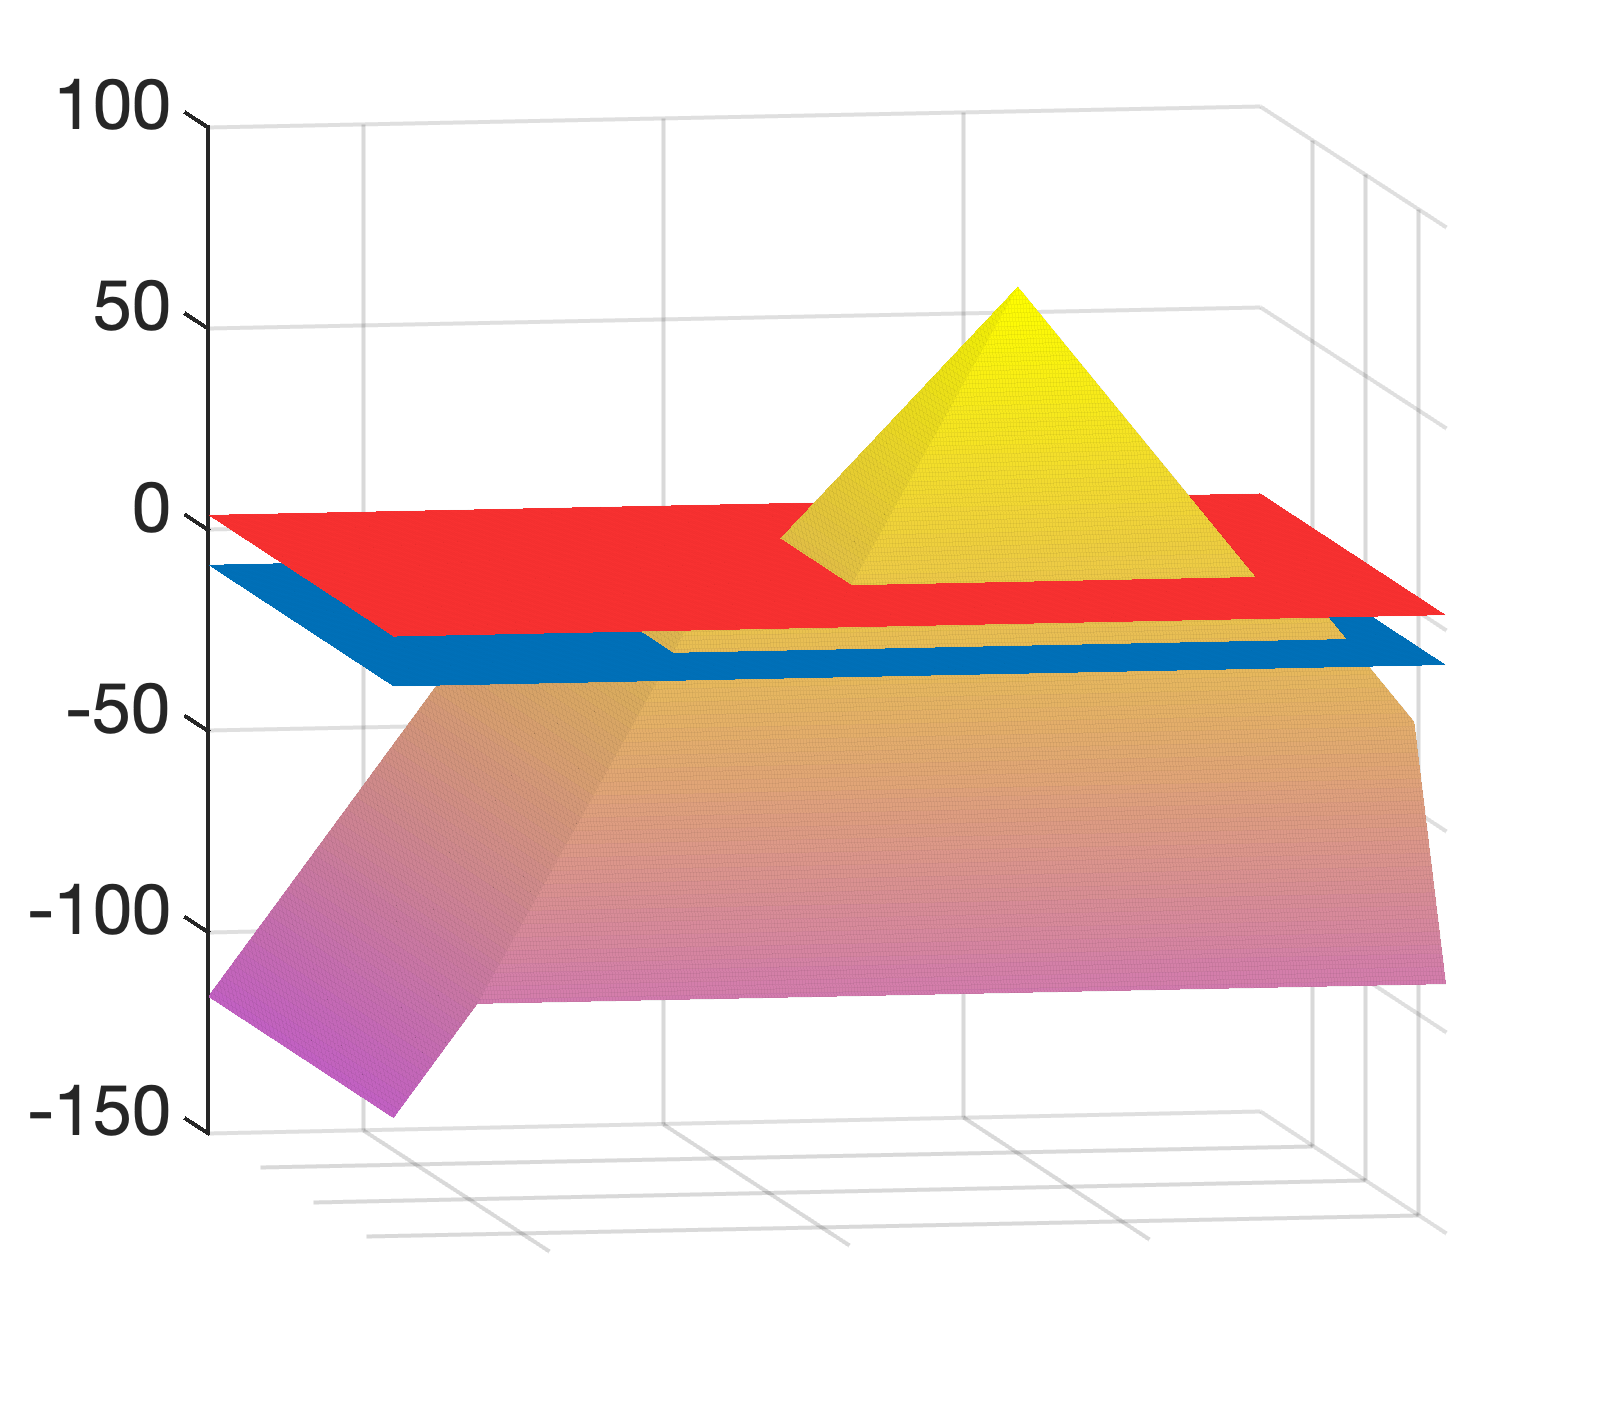
\includegraphics[width=0.24\textwidth]{../figures/learning/dist_bt_surf/903.png}\\
		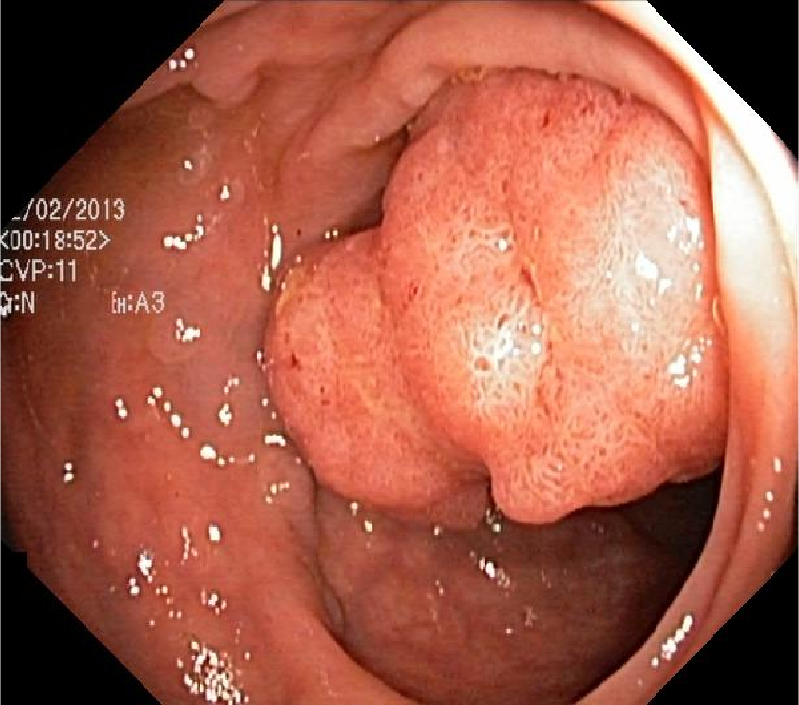
\includegraphics[width=0.24\textwidth]{../figures/learning/images/903.png}
		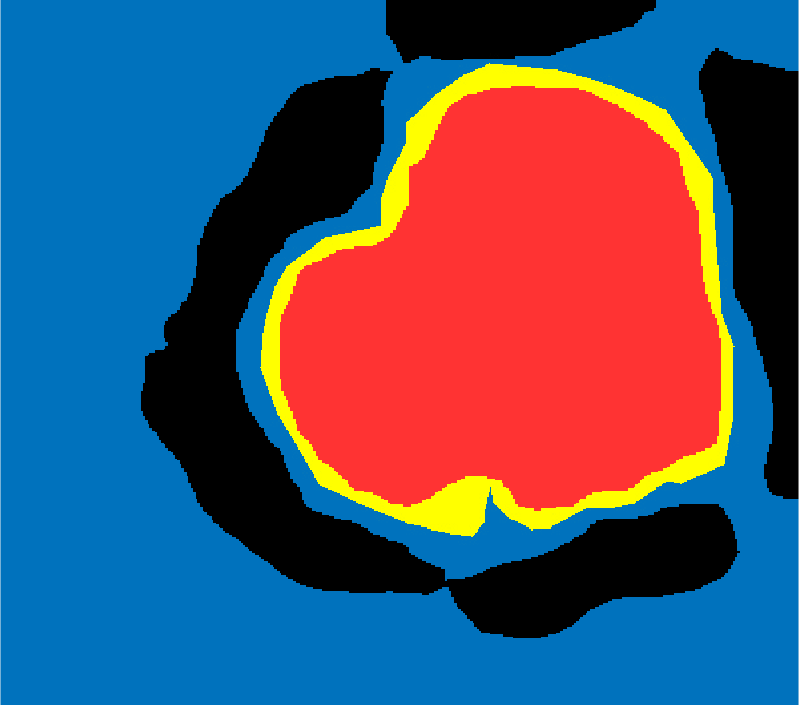
\includegraphics[width=0.24\textwidth]{../figures/learning/score_crs_marginal90/903.png}
		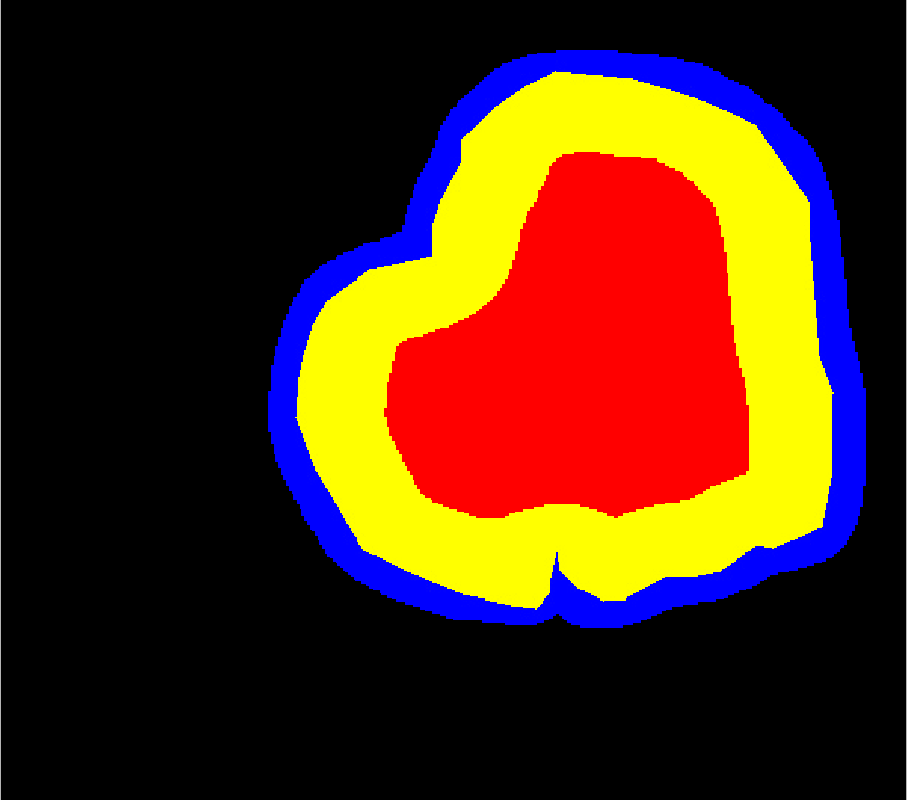
\includegraphics[width=0.24\textwidth]{../figures/learning/dist_crs_marginal90/903.png}
		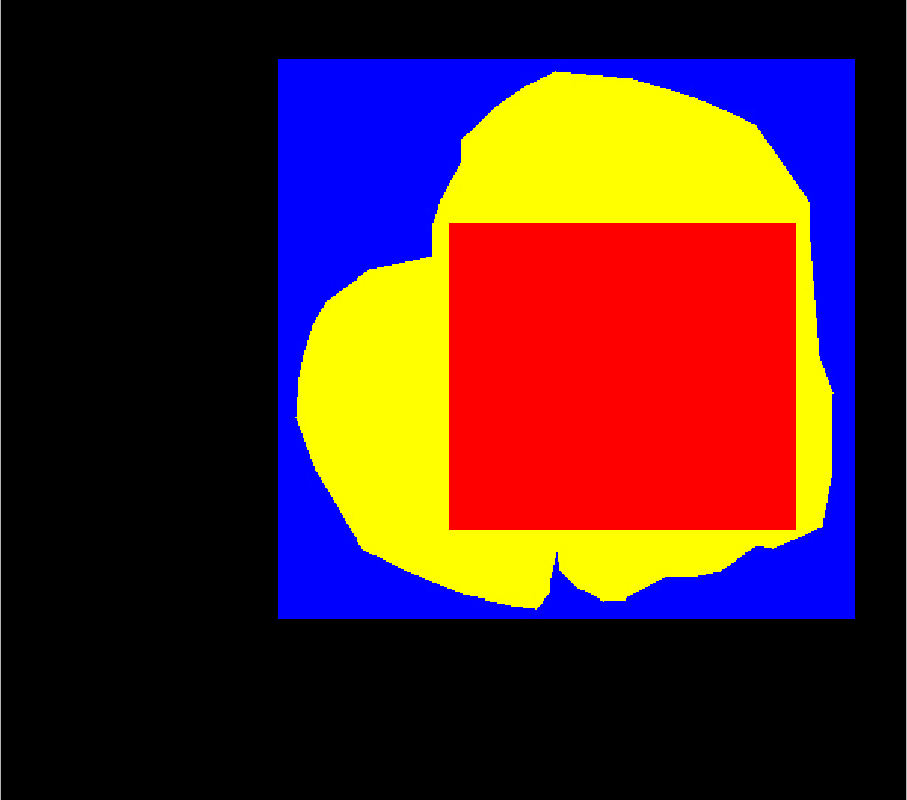
\includegraphics[width=0.24\textwidth]{../figures/learning/dist_bt_crs_marginal90/903.png}\\
			\vspace{0.5cm}
		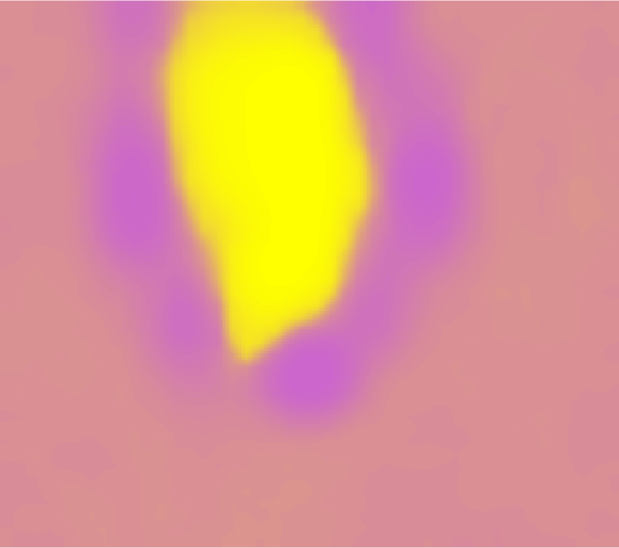
\includegraphics[width=0.24\textwidth]{../figures/learning/scores/54.png}
		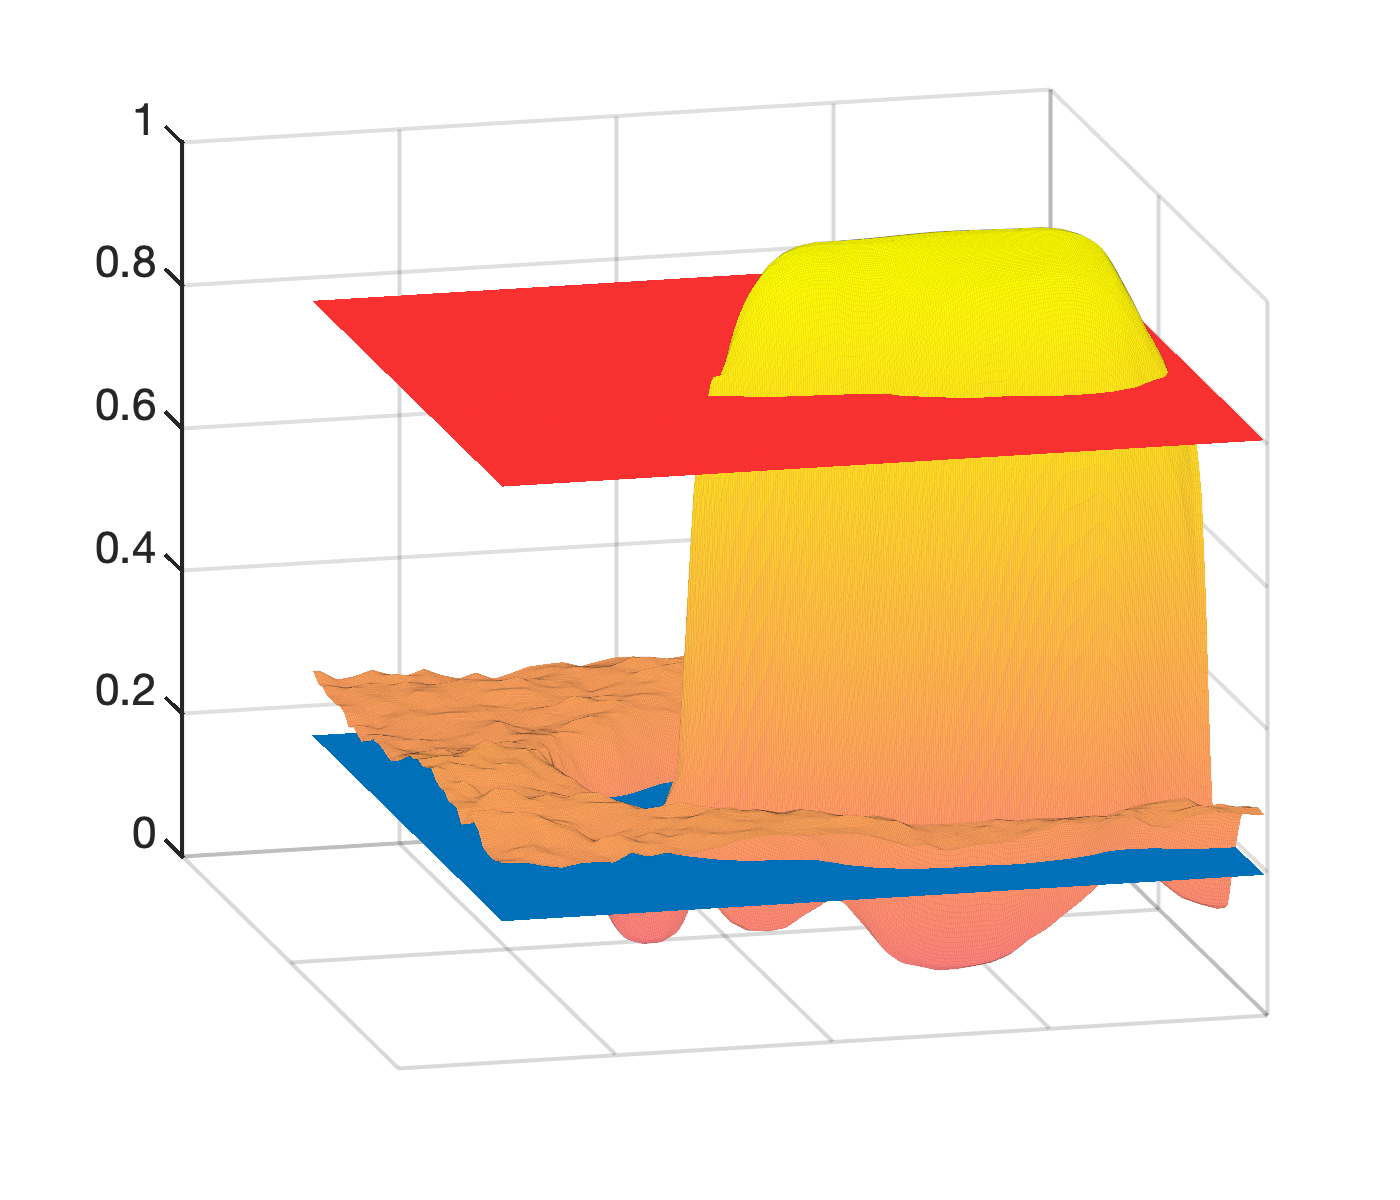
\includegraphics[width=0.24\textwidth]{../figures/learning/score_surf/54.png}	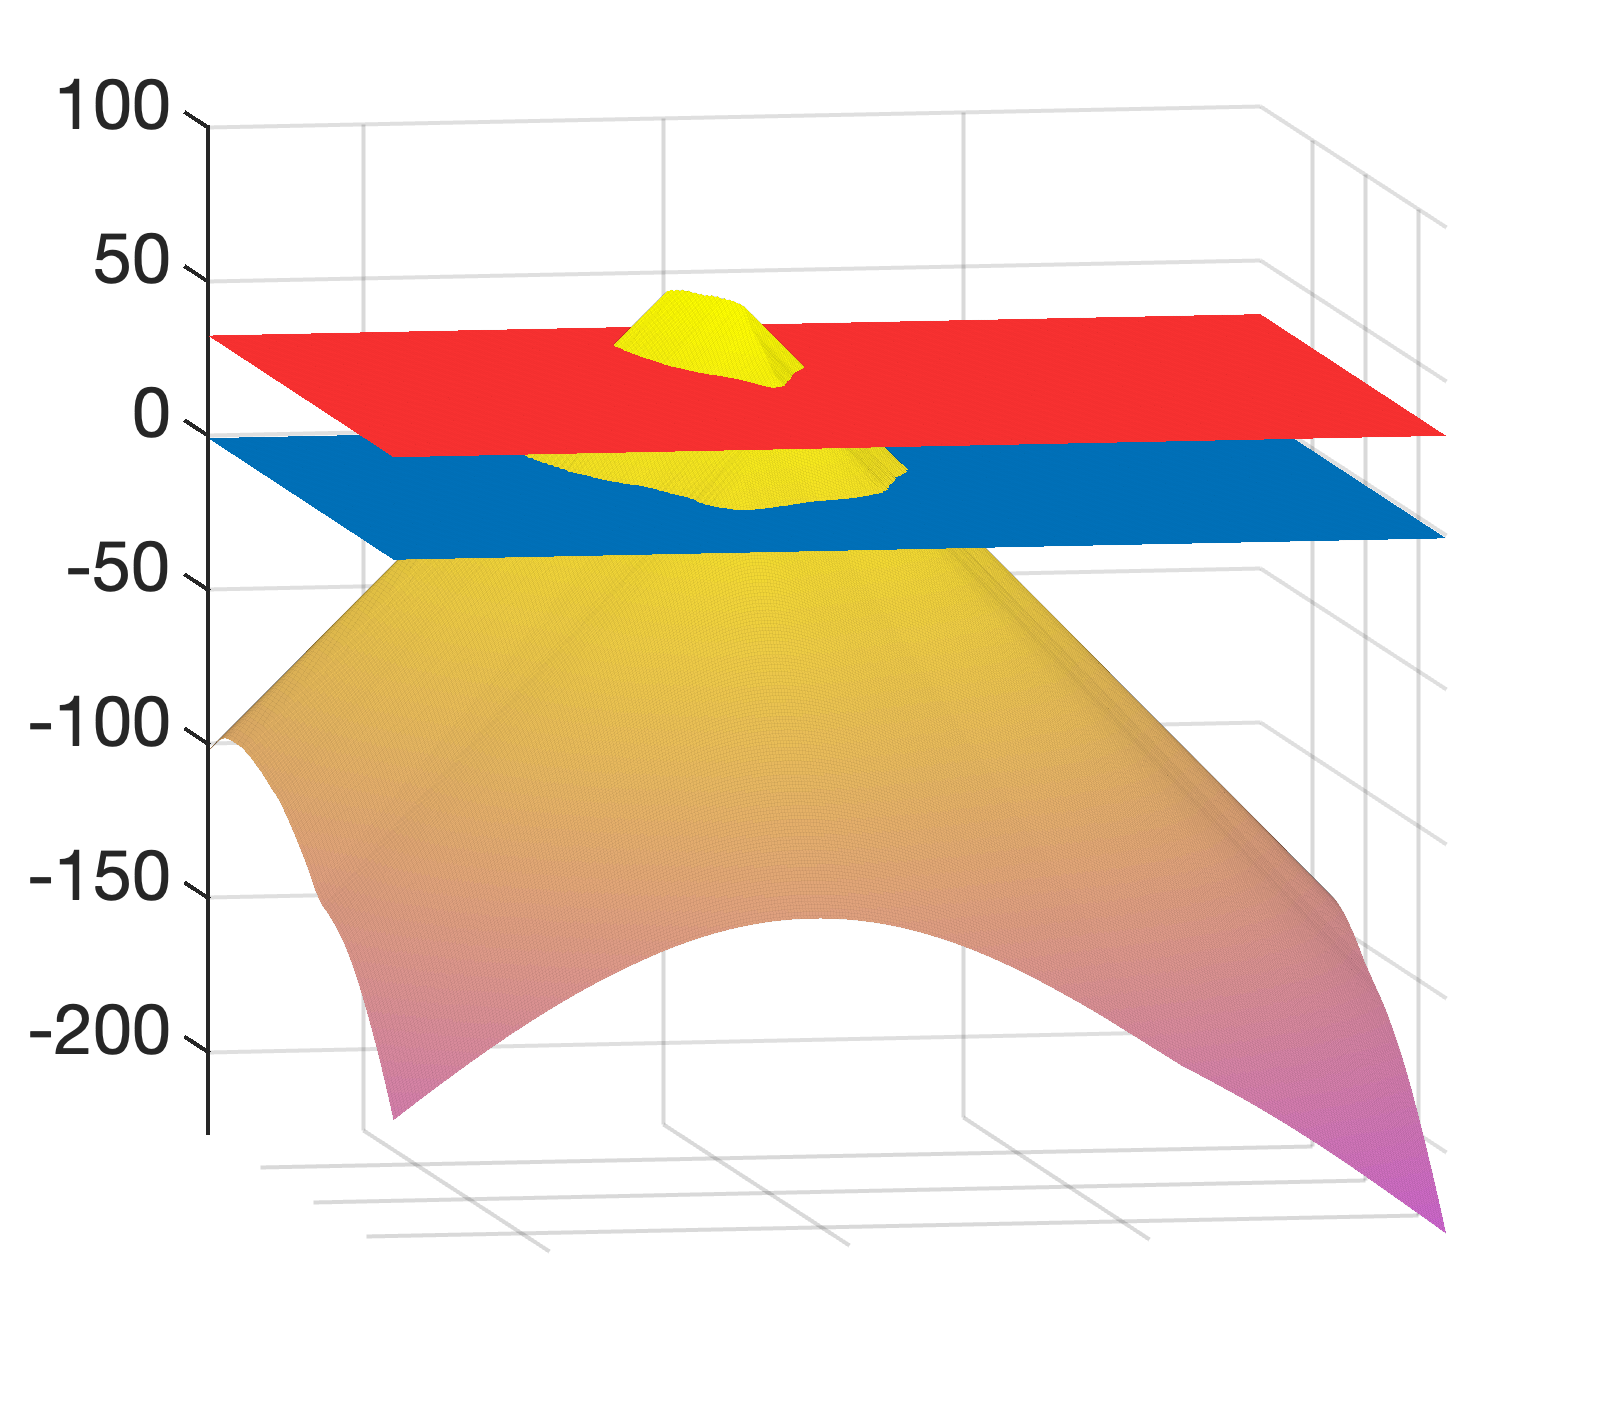
\includegraphics[width=0.24\textwidth]{../figures/learning/dist_surf/54.png}
		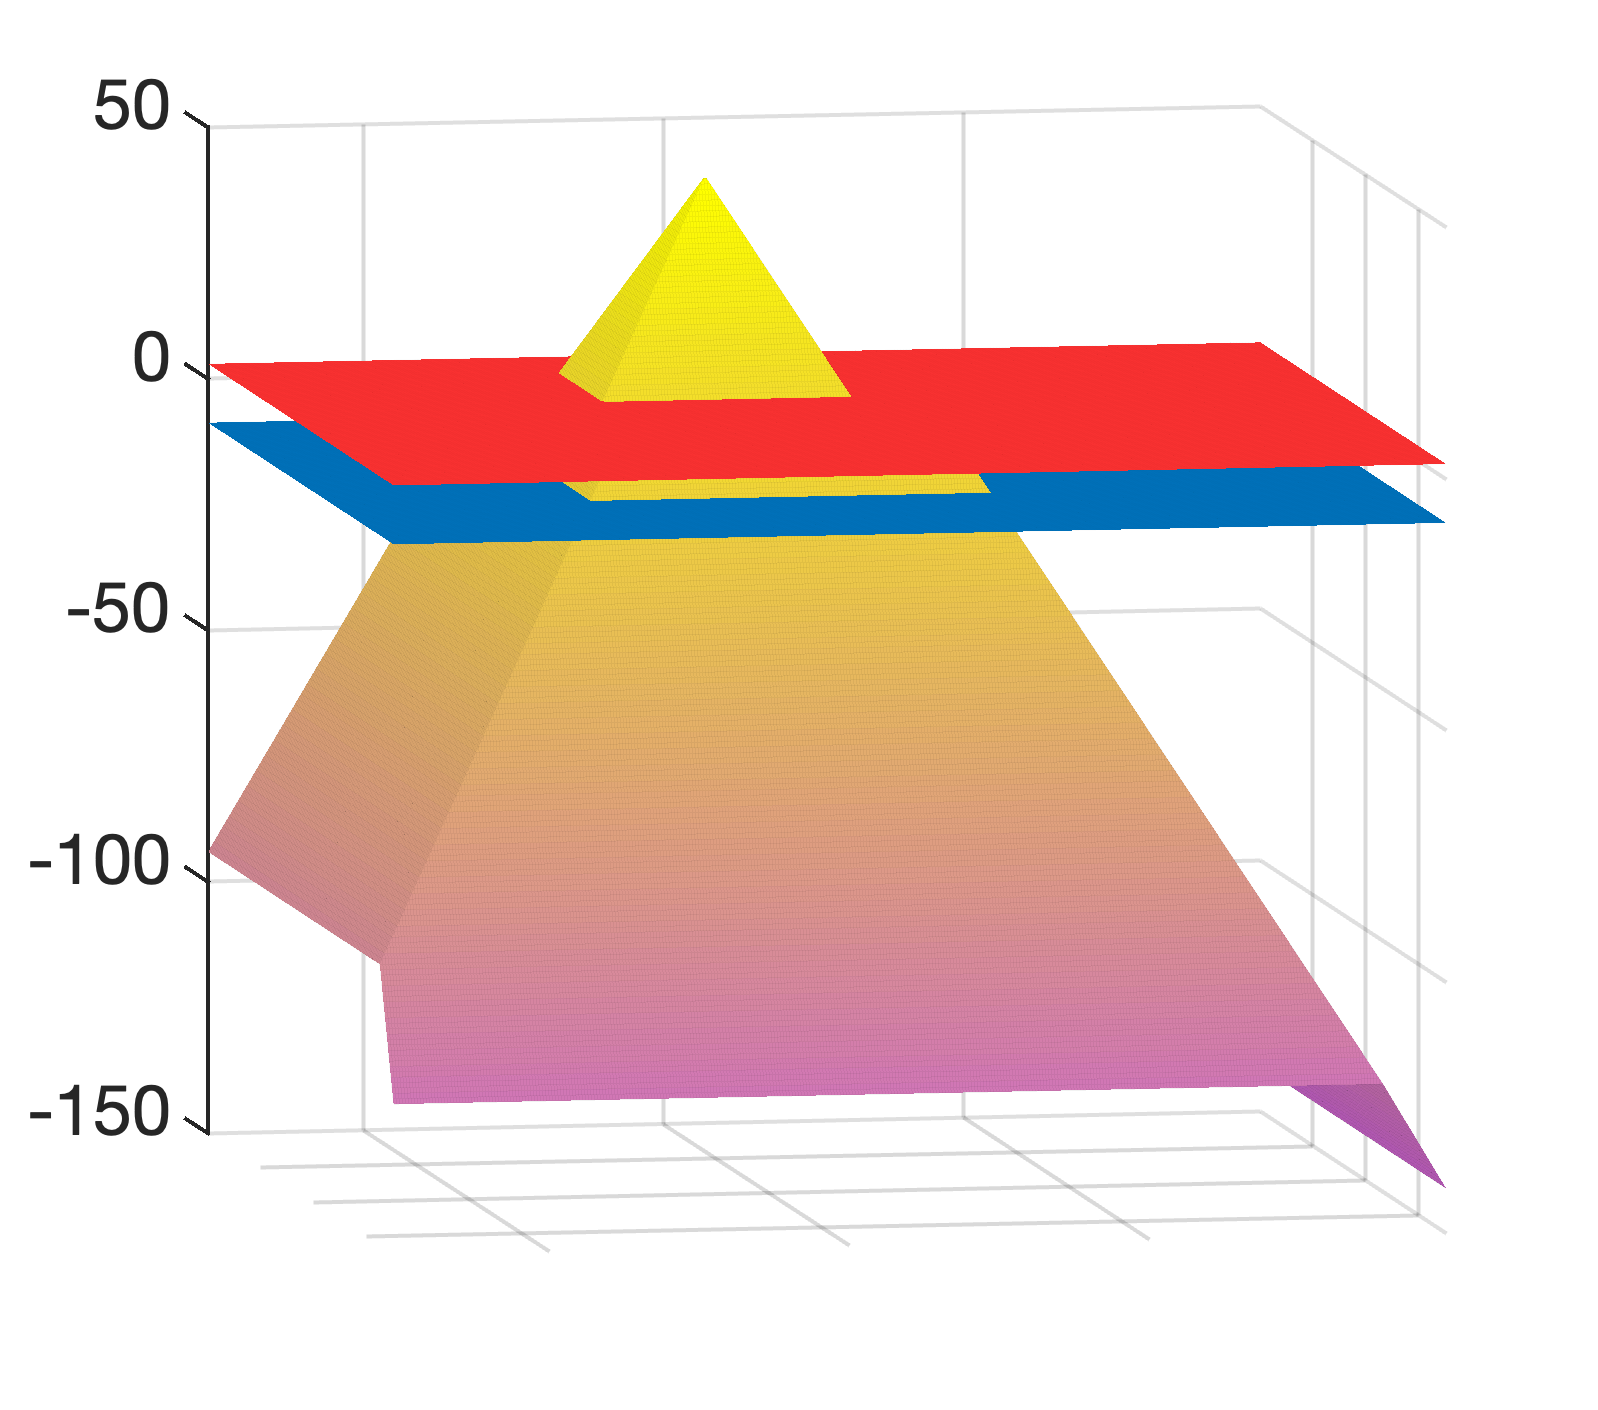
\includegraphics[width=0.24\textwidth]{../figures/learning/dist_bt_surf/54.png}\\
		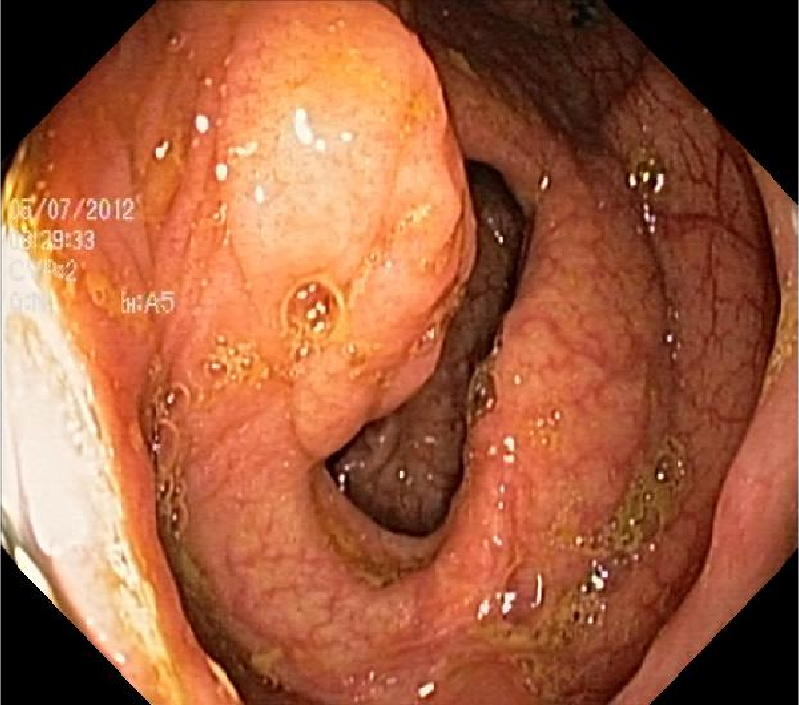
\includegraphics[width=0.24\textwidth]{../figures/learning/images/54.png}
		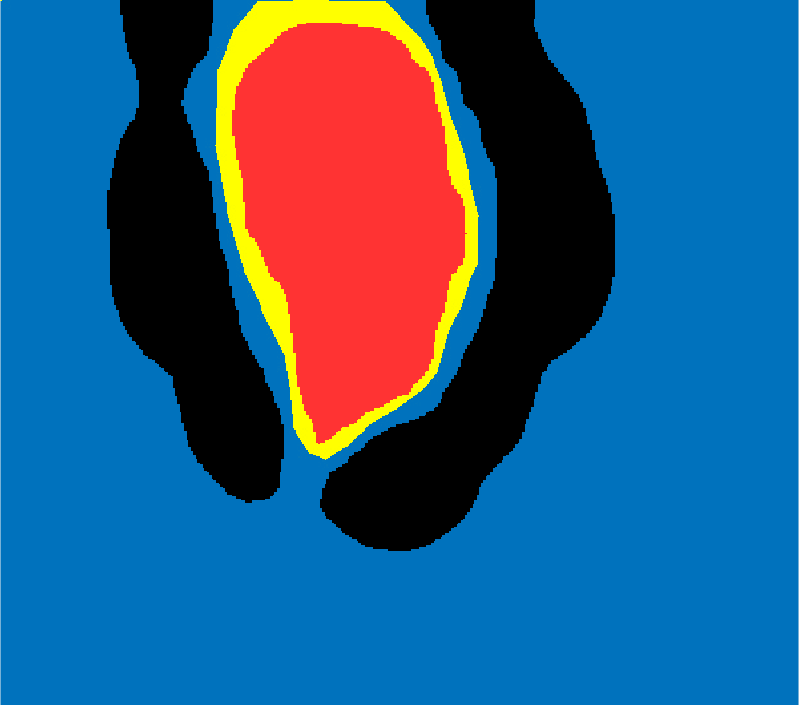
\includegraphics[width=0.24\textwidth]{../figures/learning/score_crs_marginal90/54.png}
		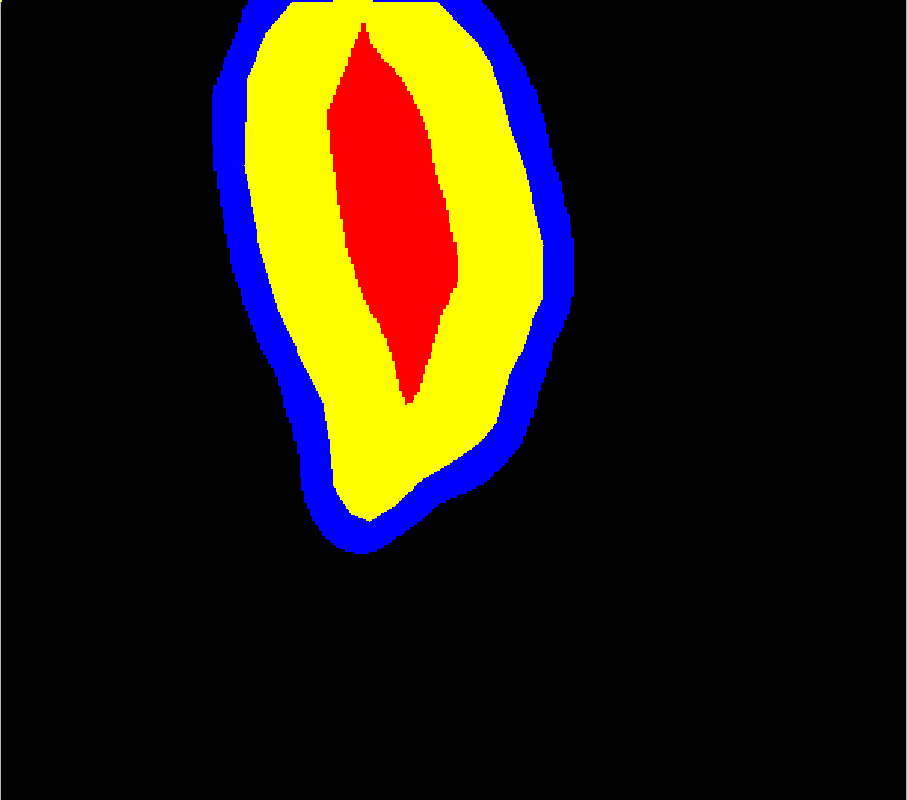
\includegraphics[width=0.24\textwidth]{../figures/learning/dist_crs_marginal90/54.png}
		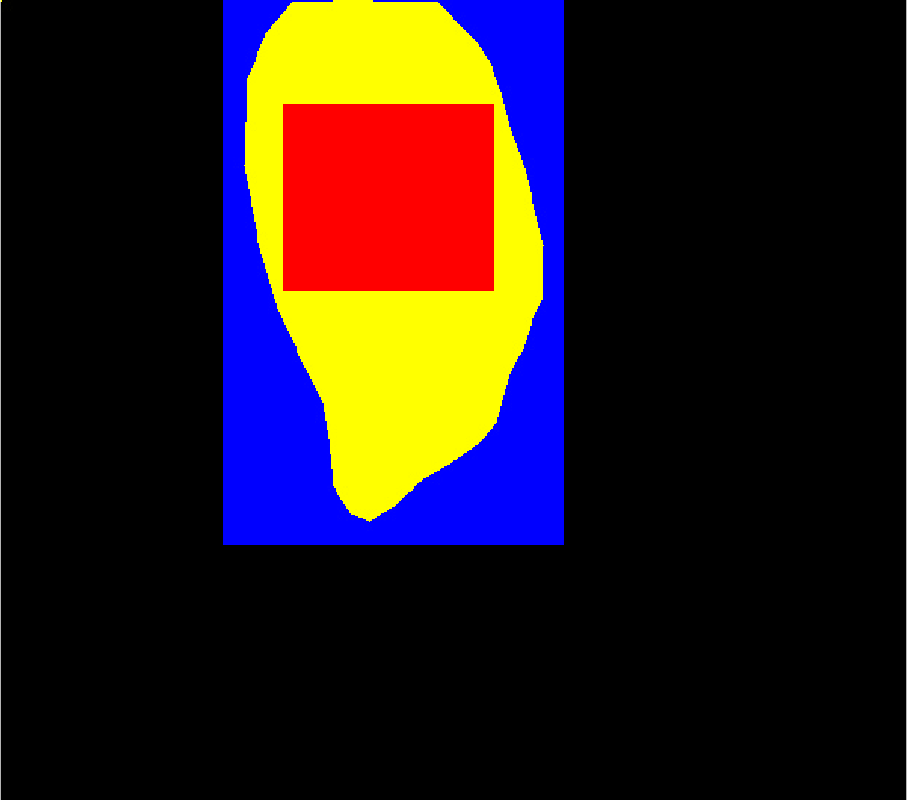
\includegraphics[width=0.24\textwidth]{../figures/learning/dist_bt_crs_marginal90/54.png}
	\end{center}
	\caption{Additional examples from the learning dataset. The layout of these figures is the same as for Figure \ref{fig:learning}.}
	\label{fig:learning2}
\end{figure}

\begin{figure}
	%	\centering
	\begin{center}
		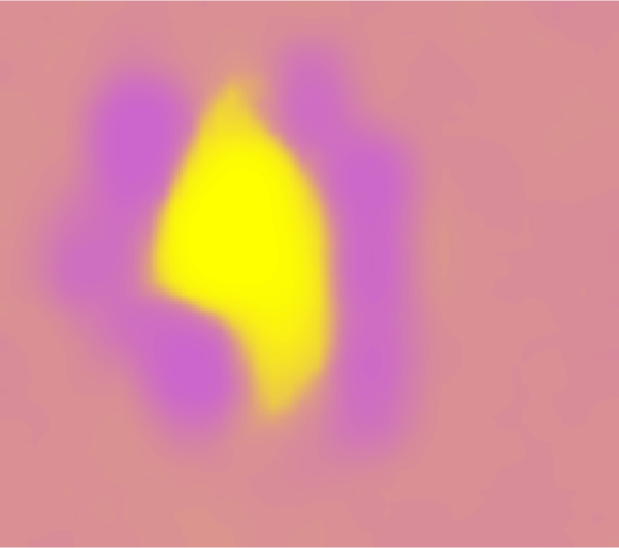
\includegraphics[width=0.24\textwidth]{../figures/learning/scores/183.png}
		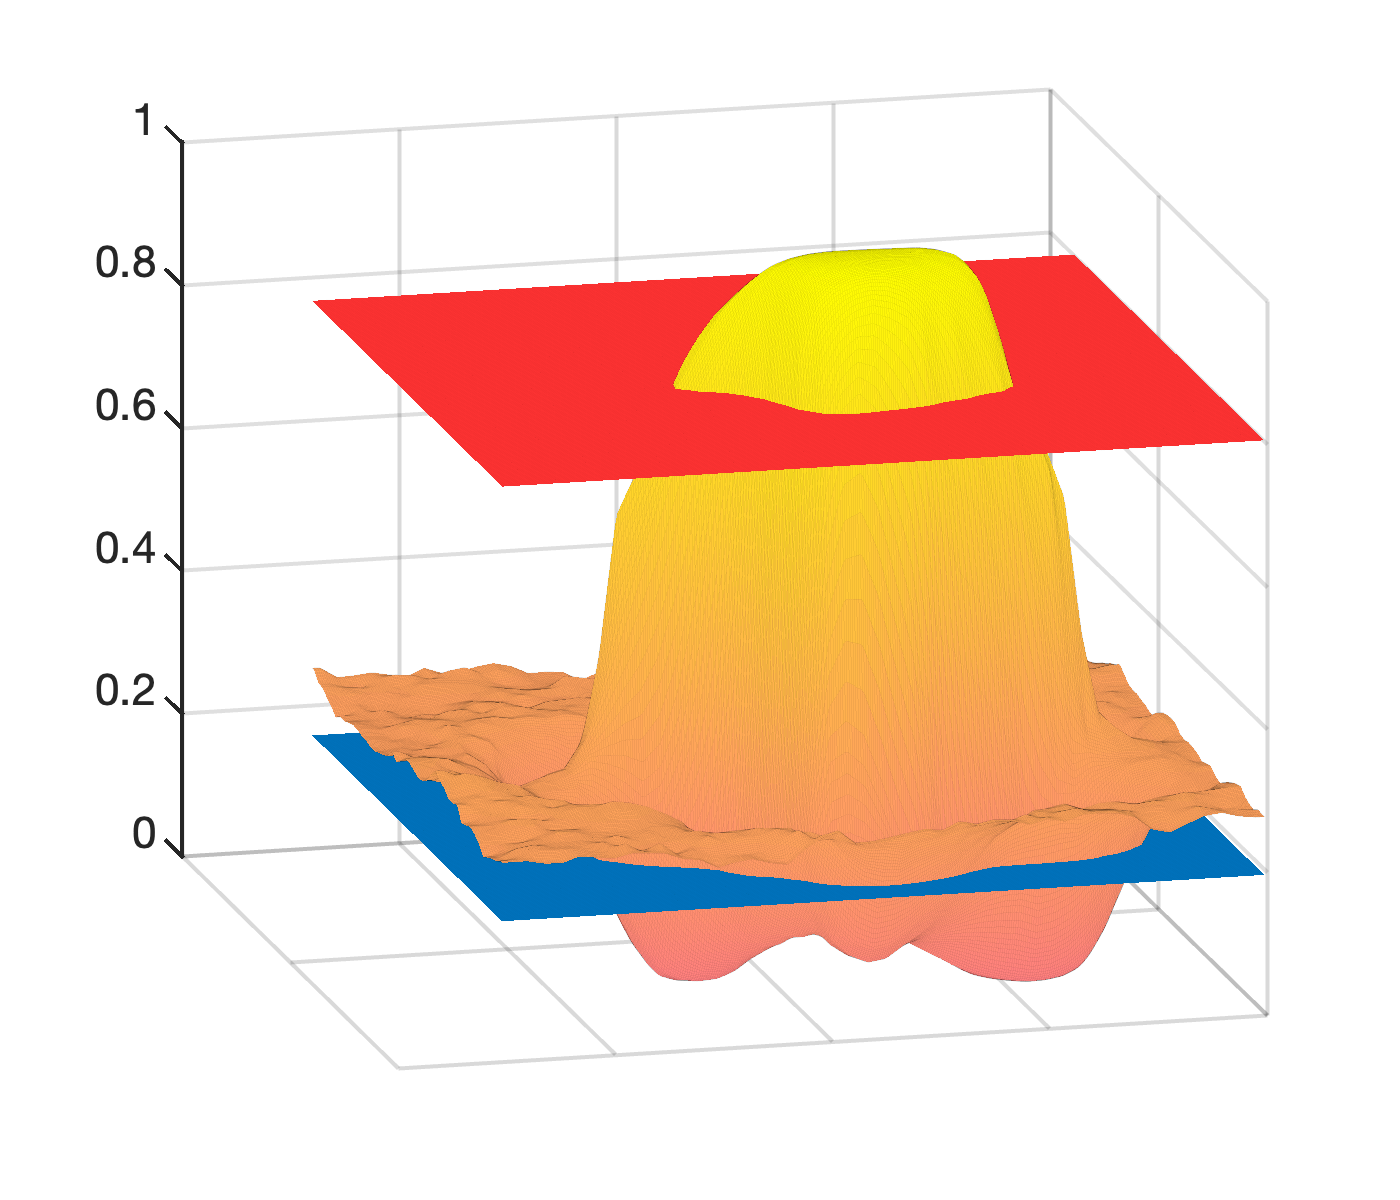
\includegraphics[width=0.24\textwidth]{../figures/learning/score_surf/183.png}	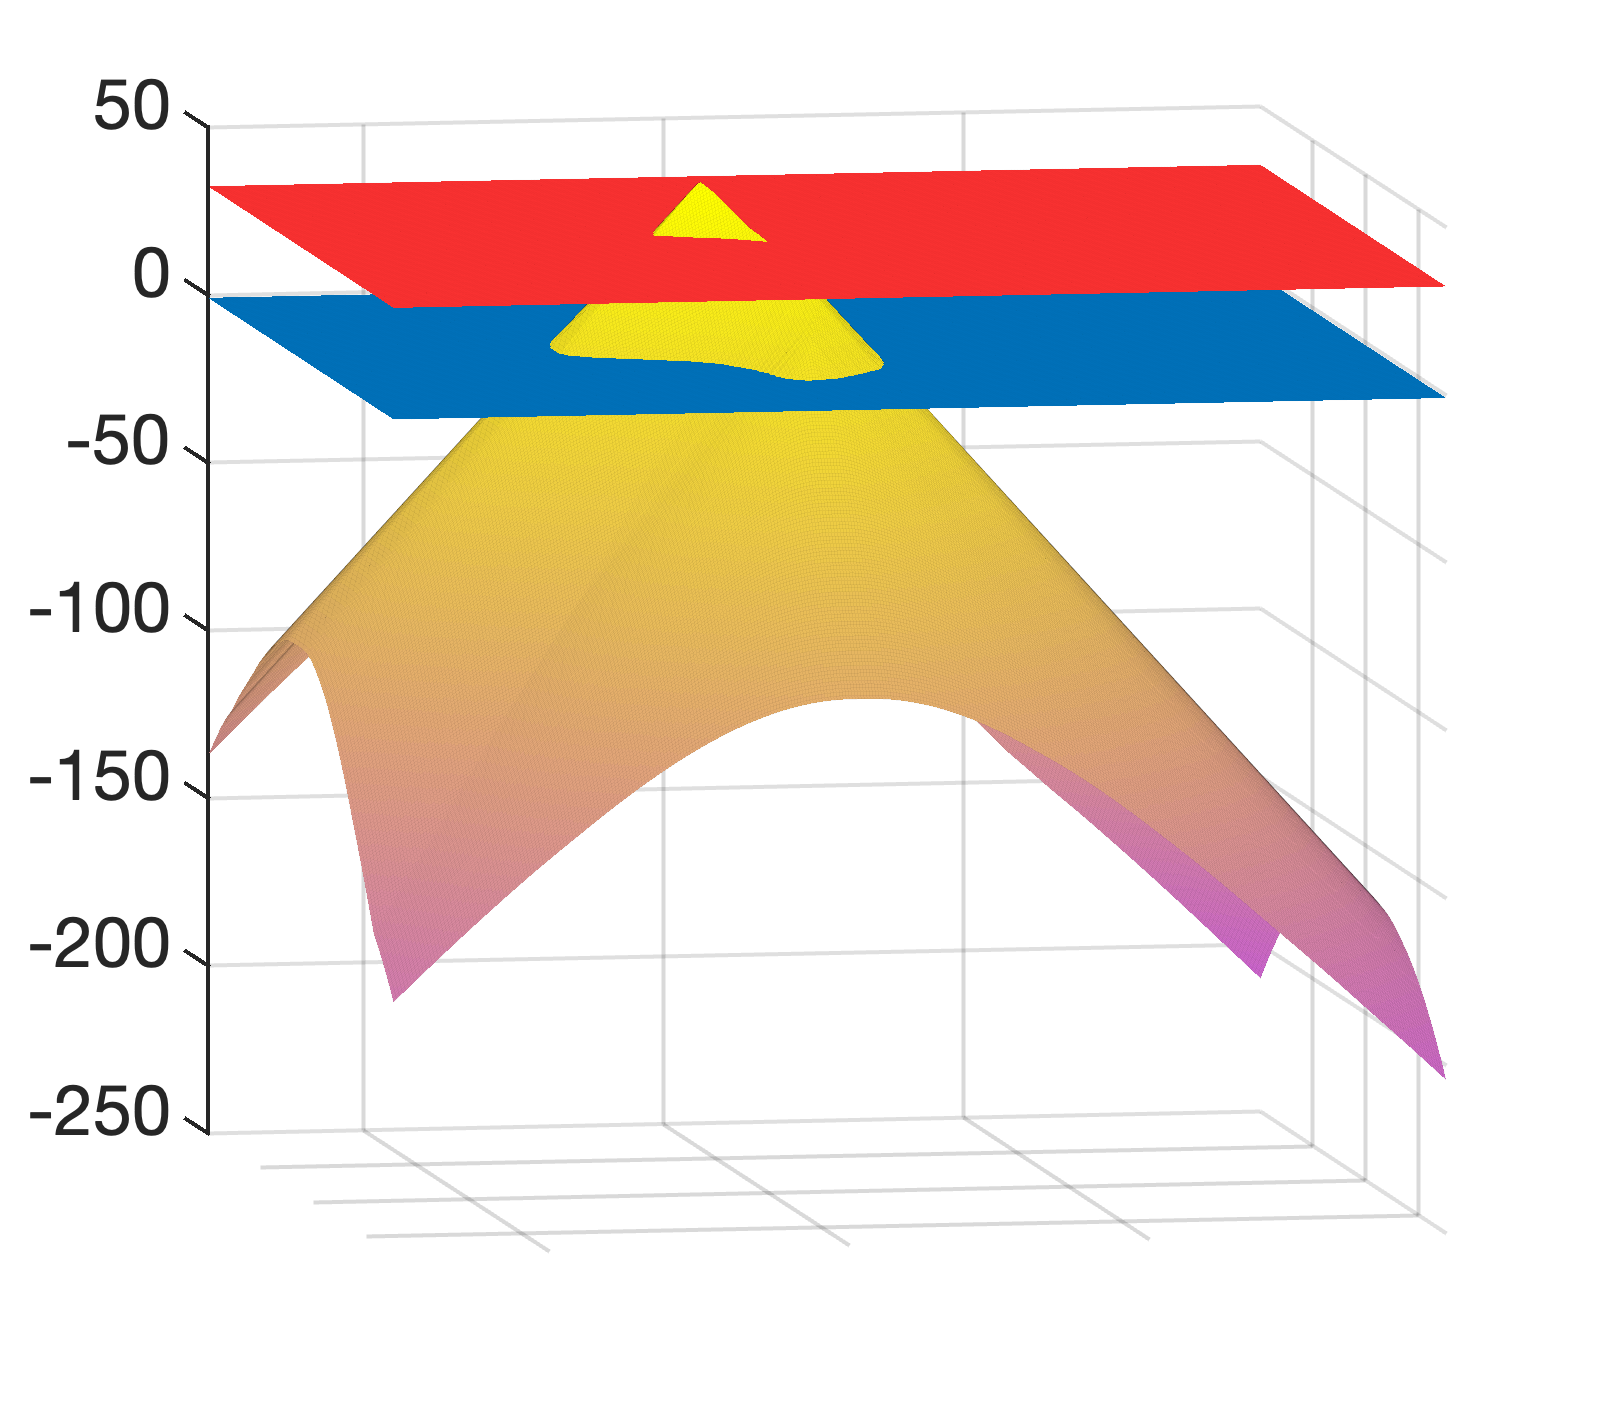
\includegraphics[width=0.24\textwidth]{../figures/learning/dist_surf/183.png}
		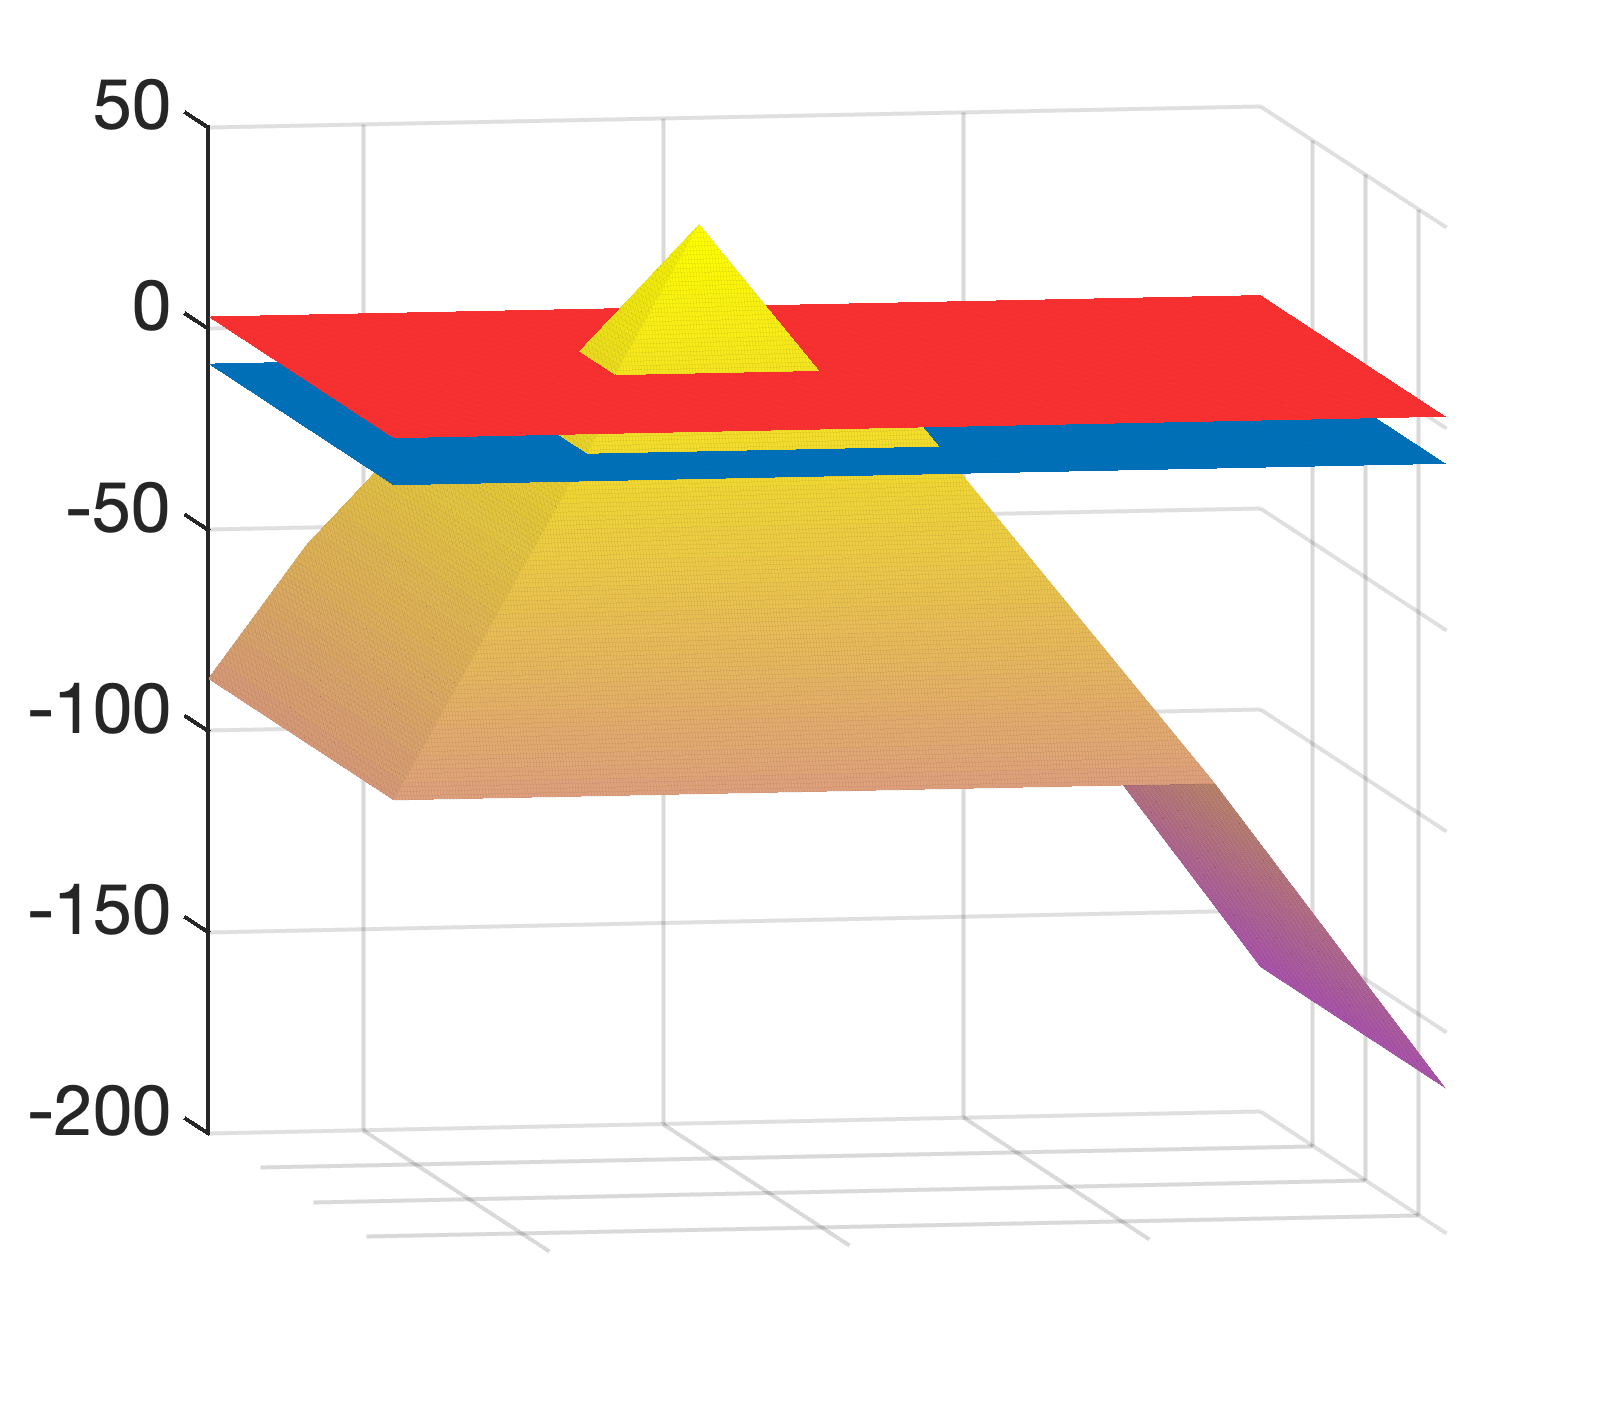
\includegraphics[width=0.24\textwidth]{../figures/learning/dist_bt_surf/183.png}\\
		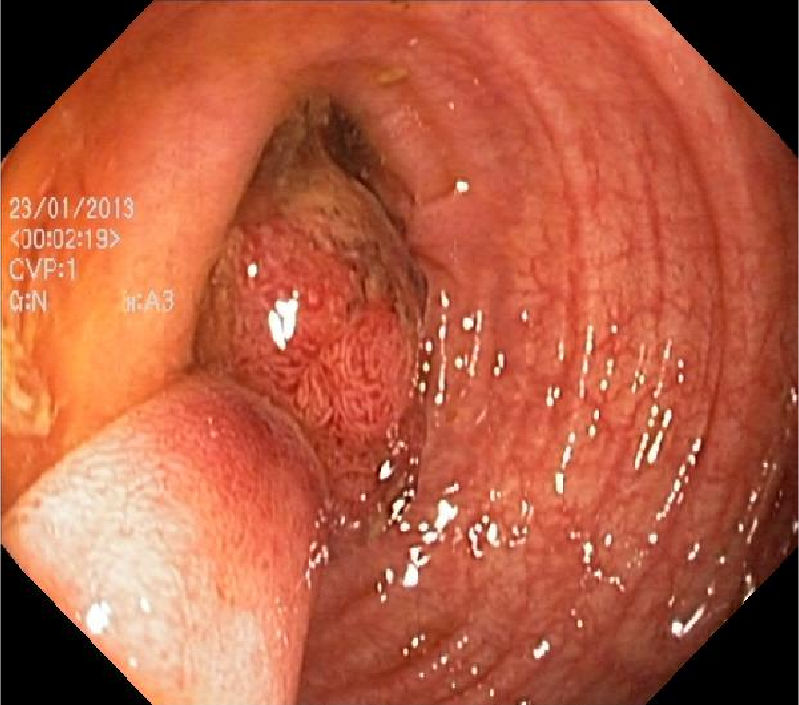
\includegraphics[width=0.24\textwidth]{../figures/learning/images/183.png}
		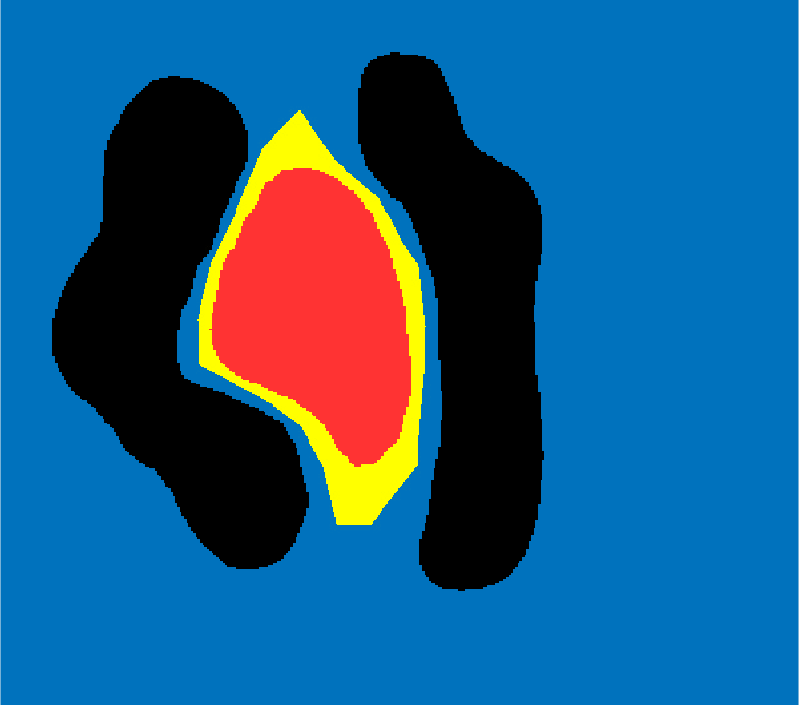
\includegraphics[width=0.24\textwidth]{../figures/learning/score_crs_marginal90/183.png}
		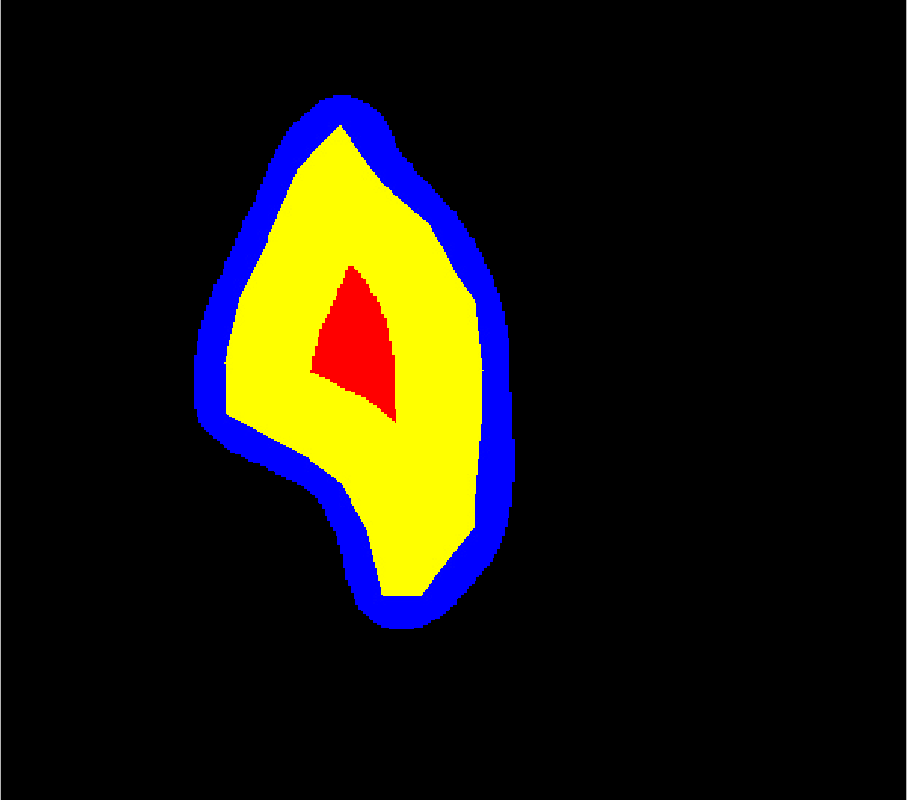
\includegraphics[width=0.24\textwidth]{../figures/learning/dist_crs_marginal90/183.png}
		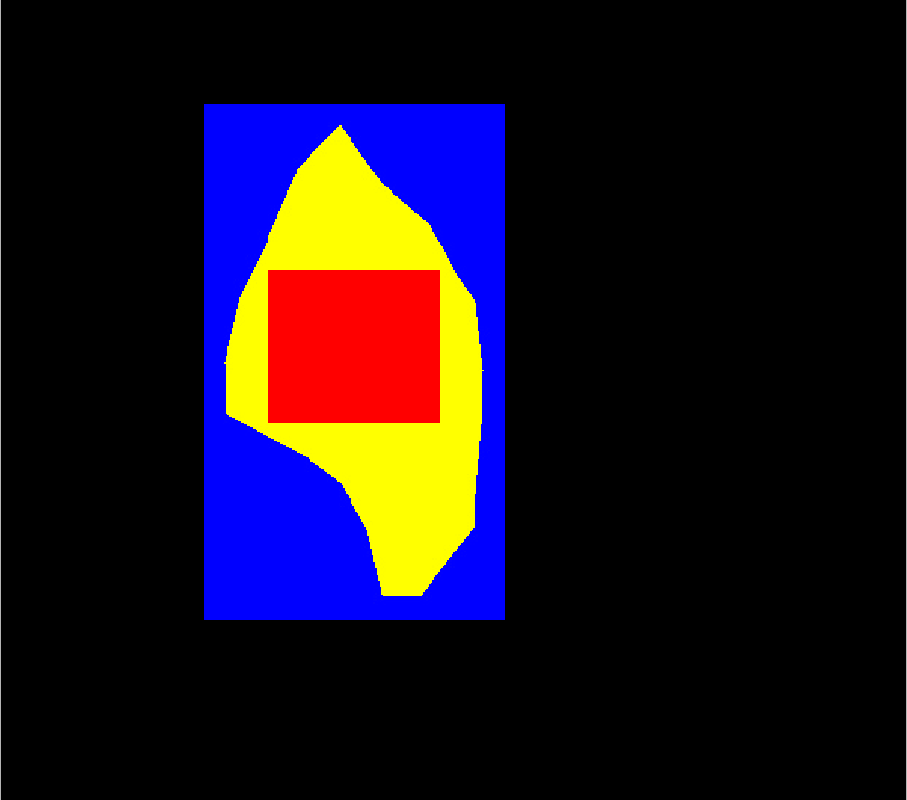
\includegraphics[width=0.24\textwidth]{../figures/learning/dist_bt_crs_marginal90/183.png}\\
		\vspace{0.5cm}
		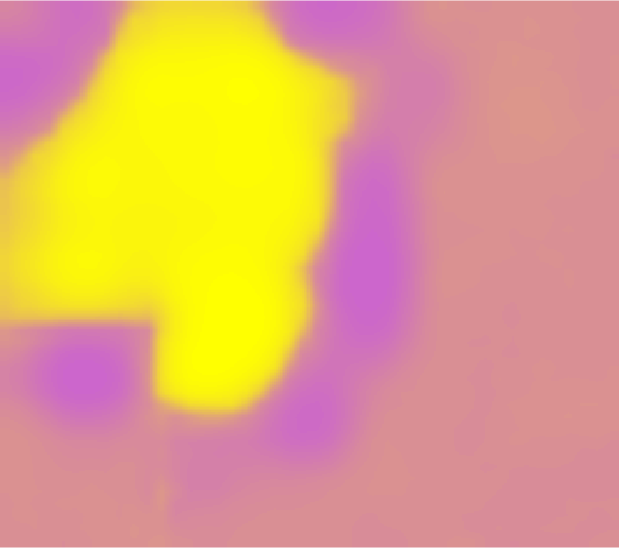
\includegraphics[width=0.24\textwidth]{../figures/learning/scores/530.png}
		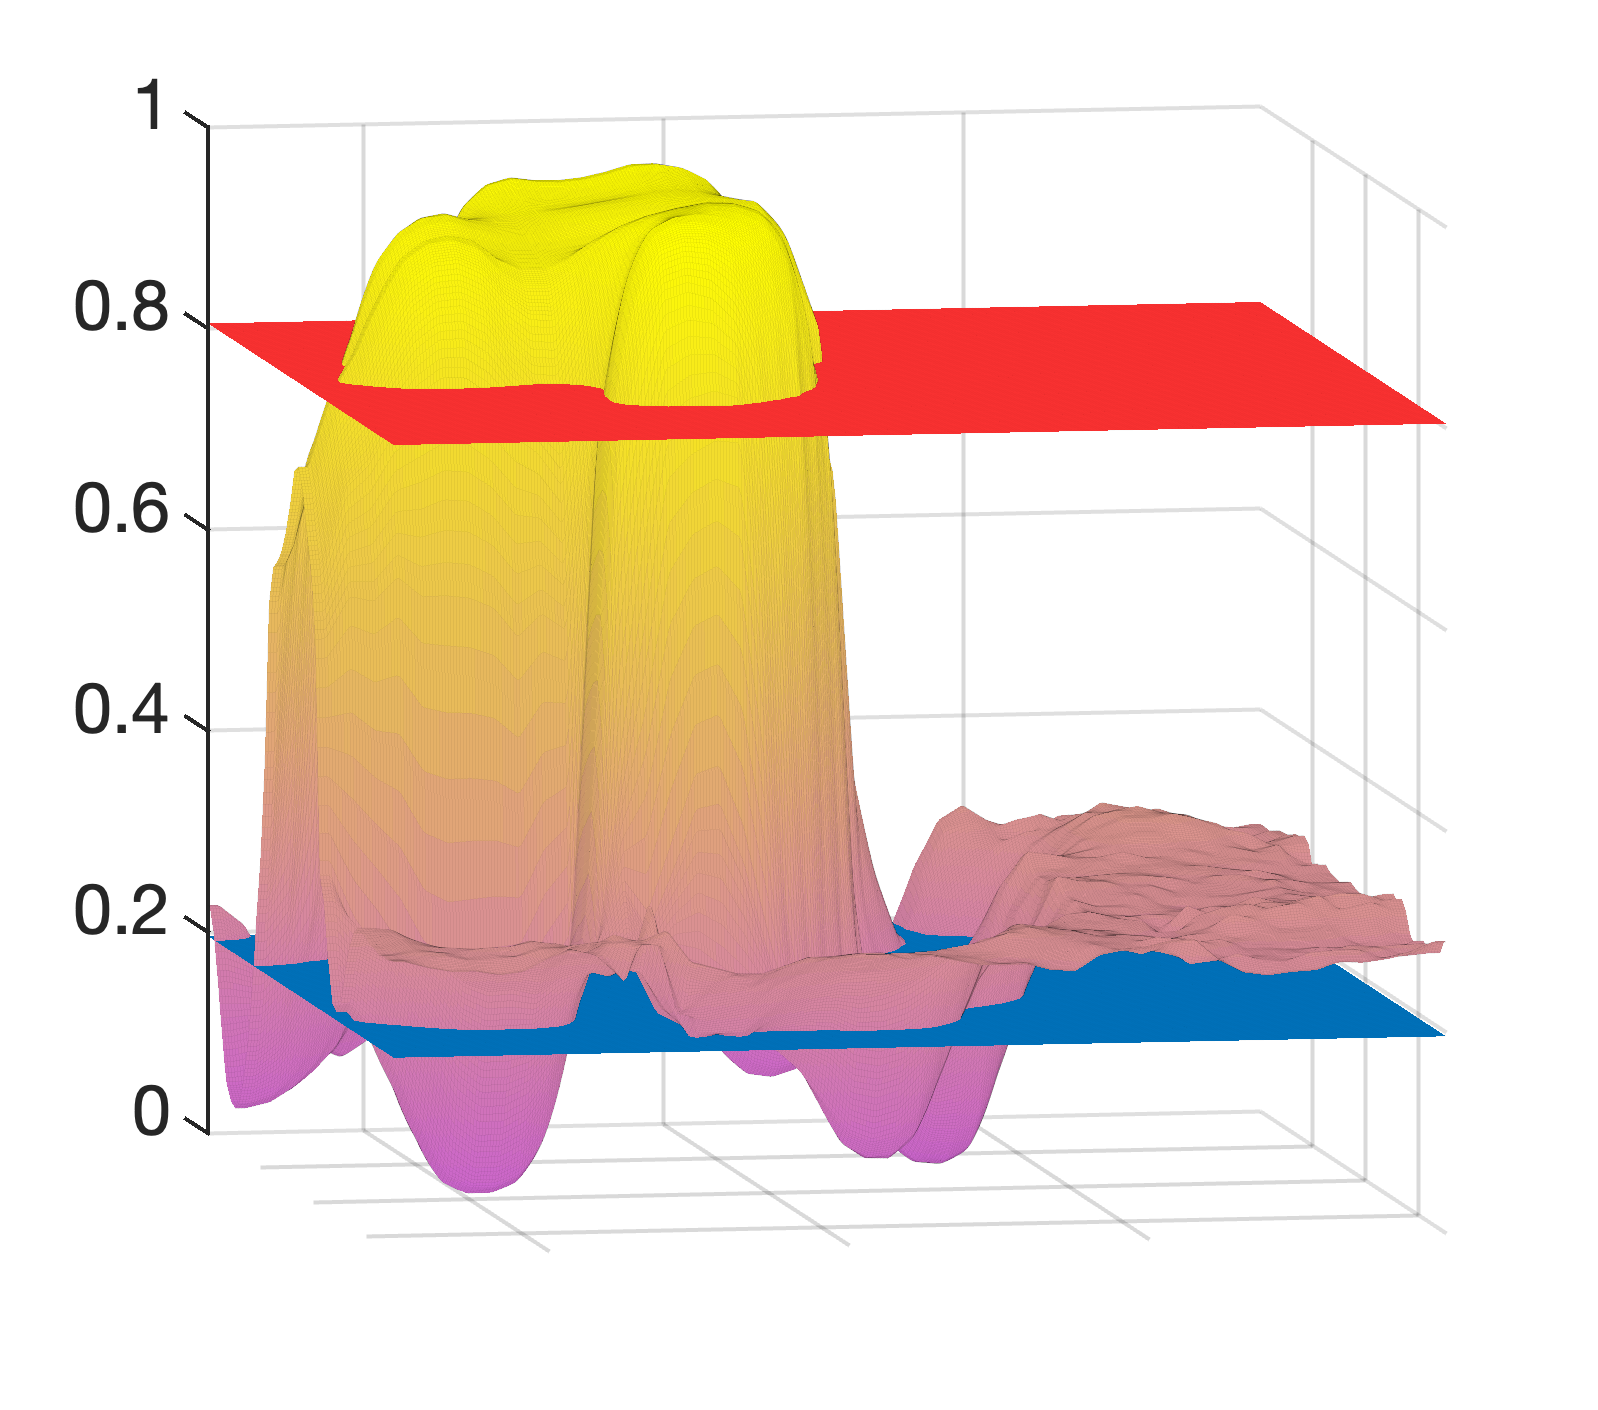
\includegraphics[width=0.24\textwidth]{../figures/learning/score_surf/530.png}	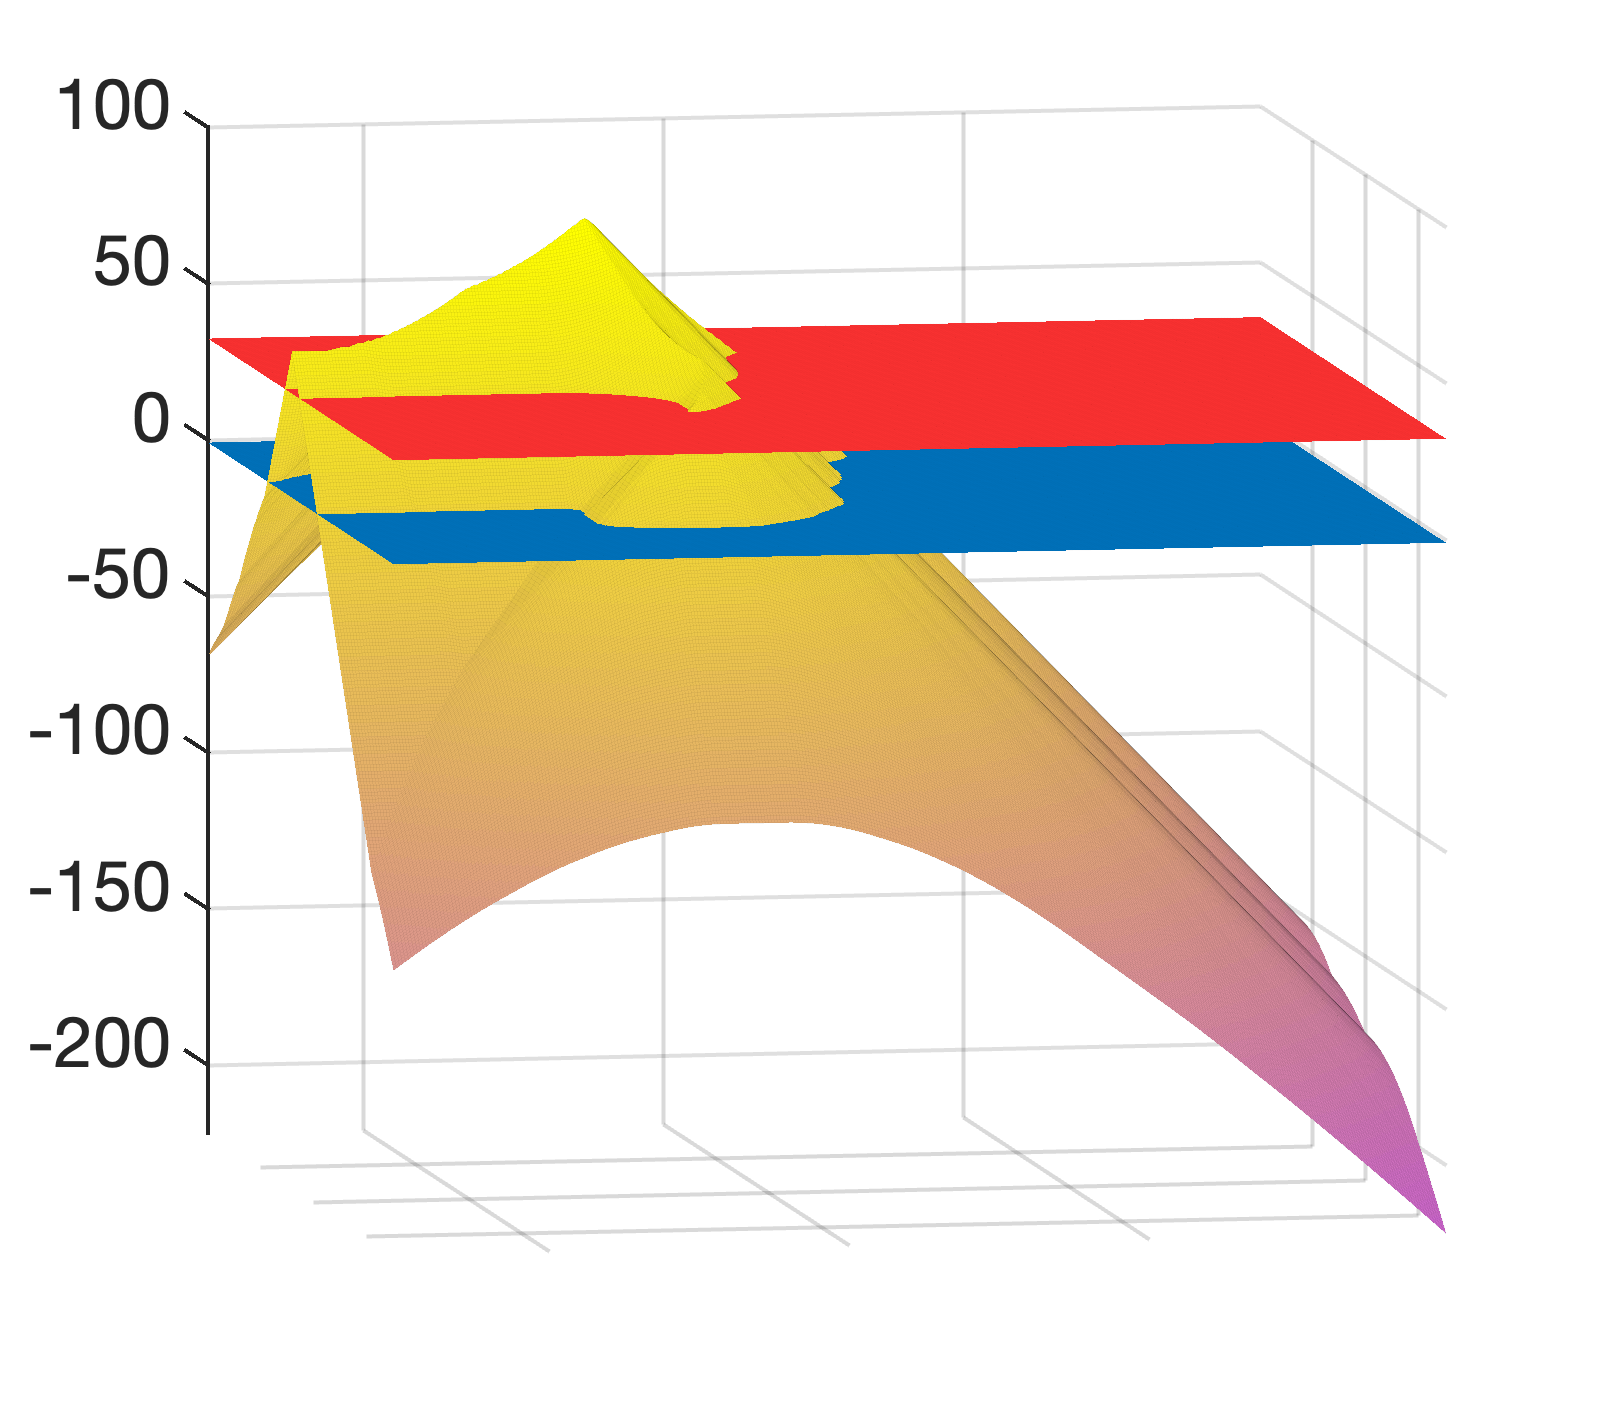
\includegraphics[width=0.24\textwidth]{../figures/learning/dist_surf/530.png}
		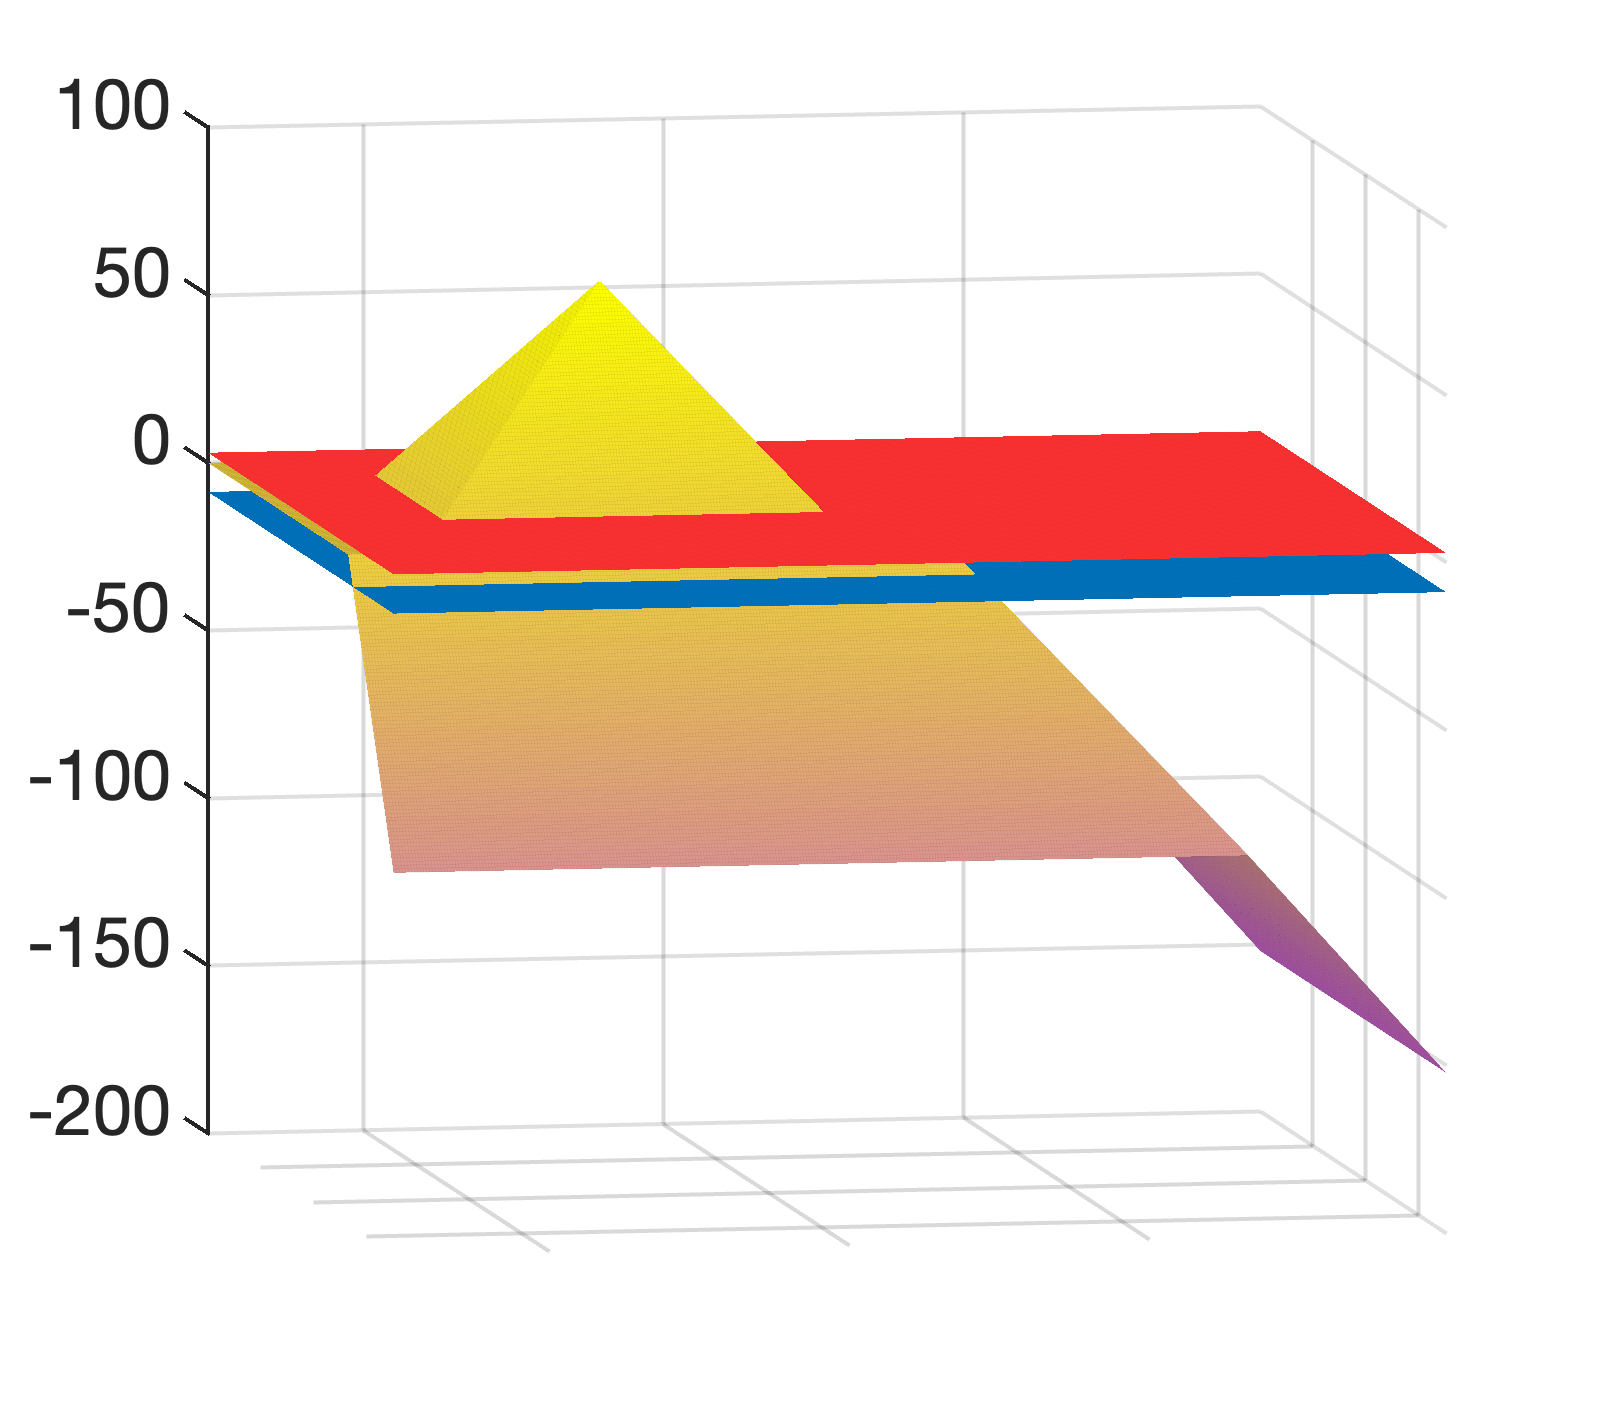
\includegraphics[width=0.24\textwidth]{../figures/learning/dist_bt_surf/530.png}\\
		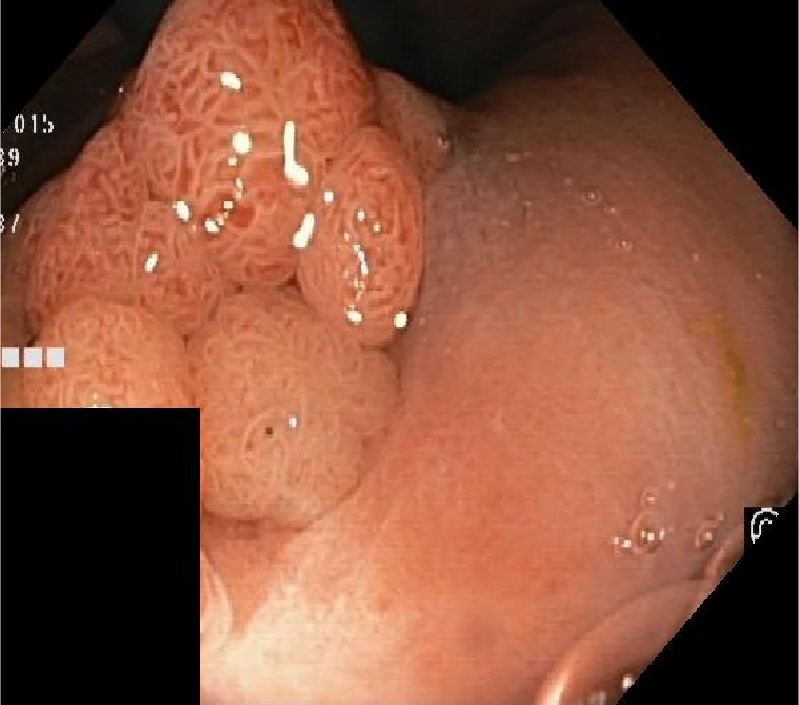
\includegraphics[width=0.24\textwidth]{../figures/learning/images/530.png}
		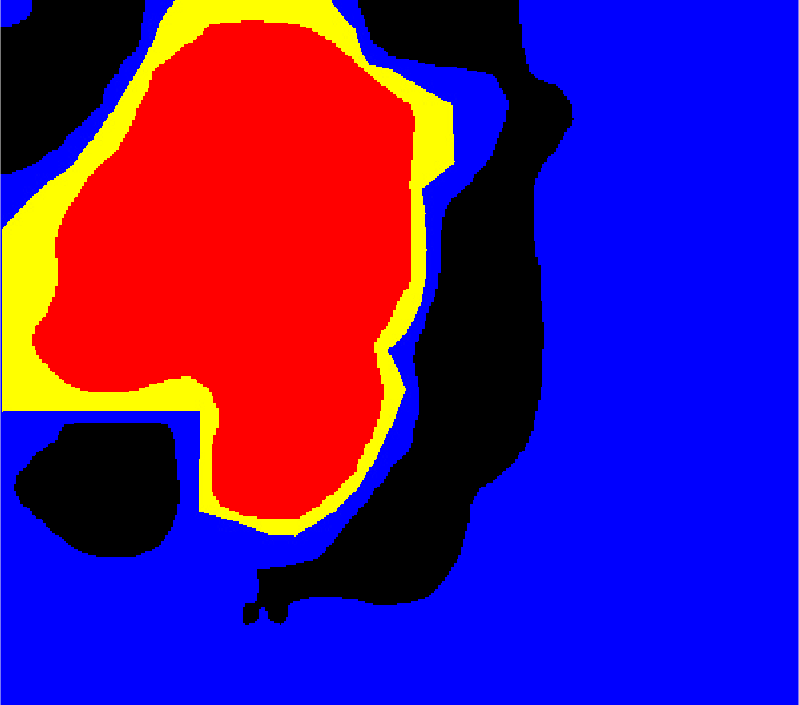
\includegraphics[width=0.24\textwidth]{../figures/learning/score_crs_marginal90/530.png}
		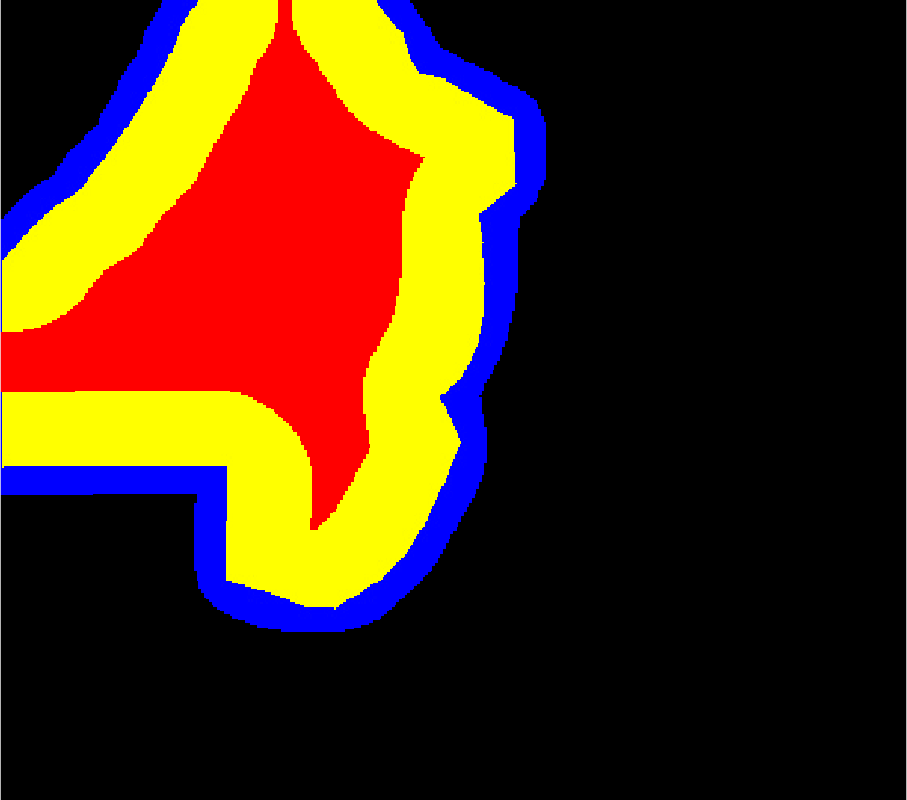
\includegraphics[width=0.24\textwidth]{../figures/learning/dist_crs_marginal90/530.png}
		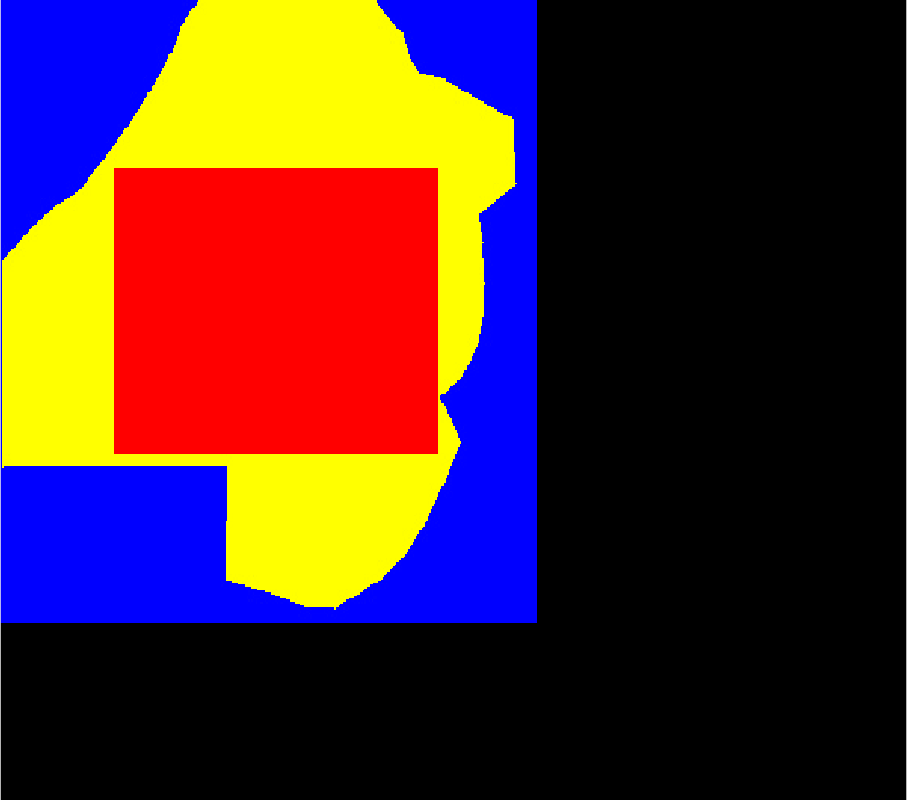
\includegraphics[width=0.24\textwidth]{../figures/learning/dist_bt_crs_marginal90/530.png}\\
		\vspace{0.5cm}
		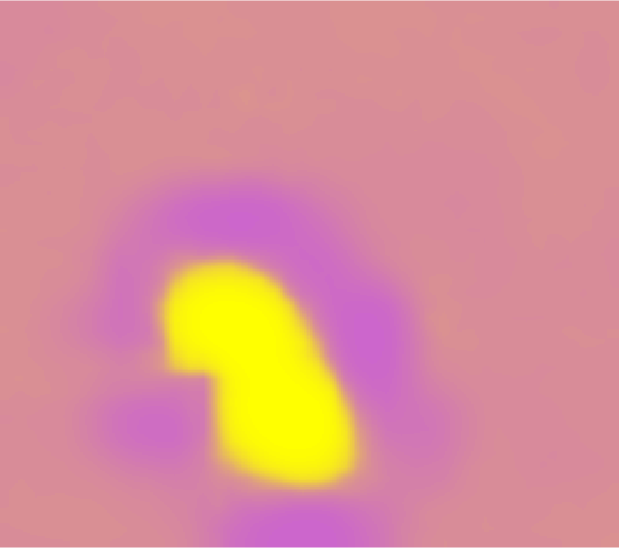
\includegraphics[width=0.24\textwidth]{../figures/learning/scores/754.png}
		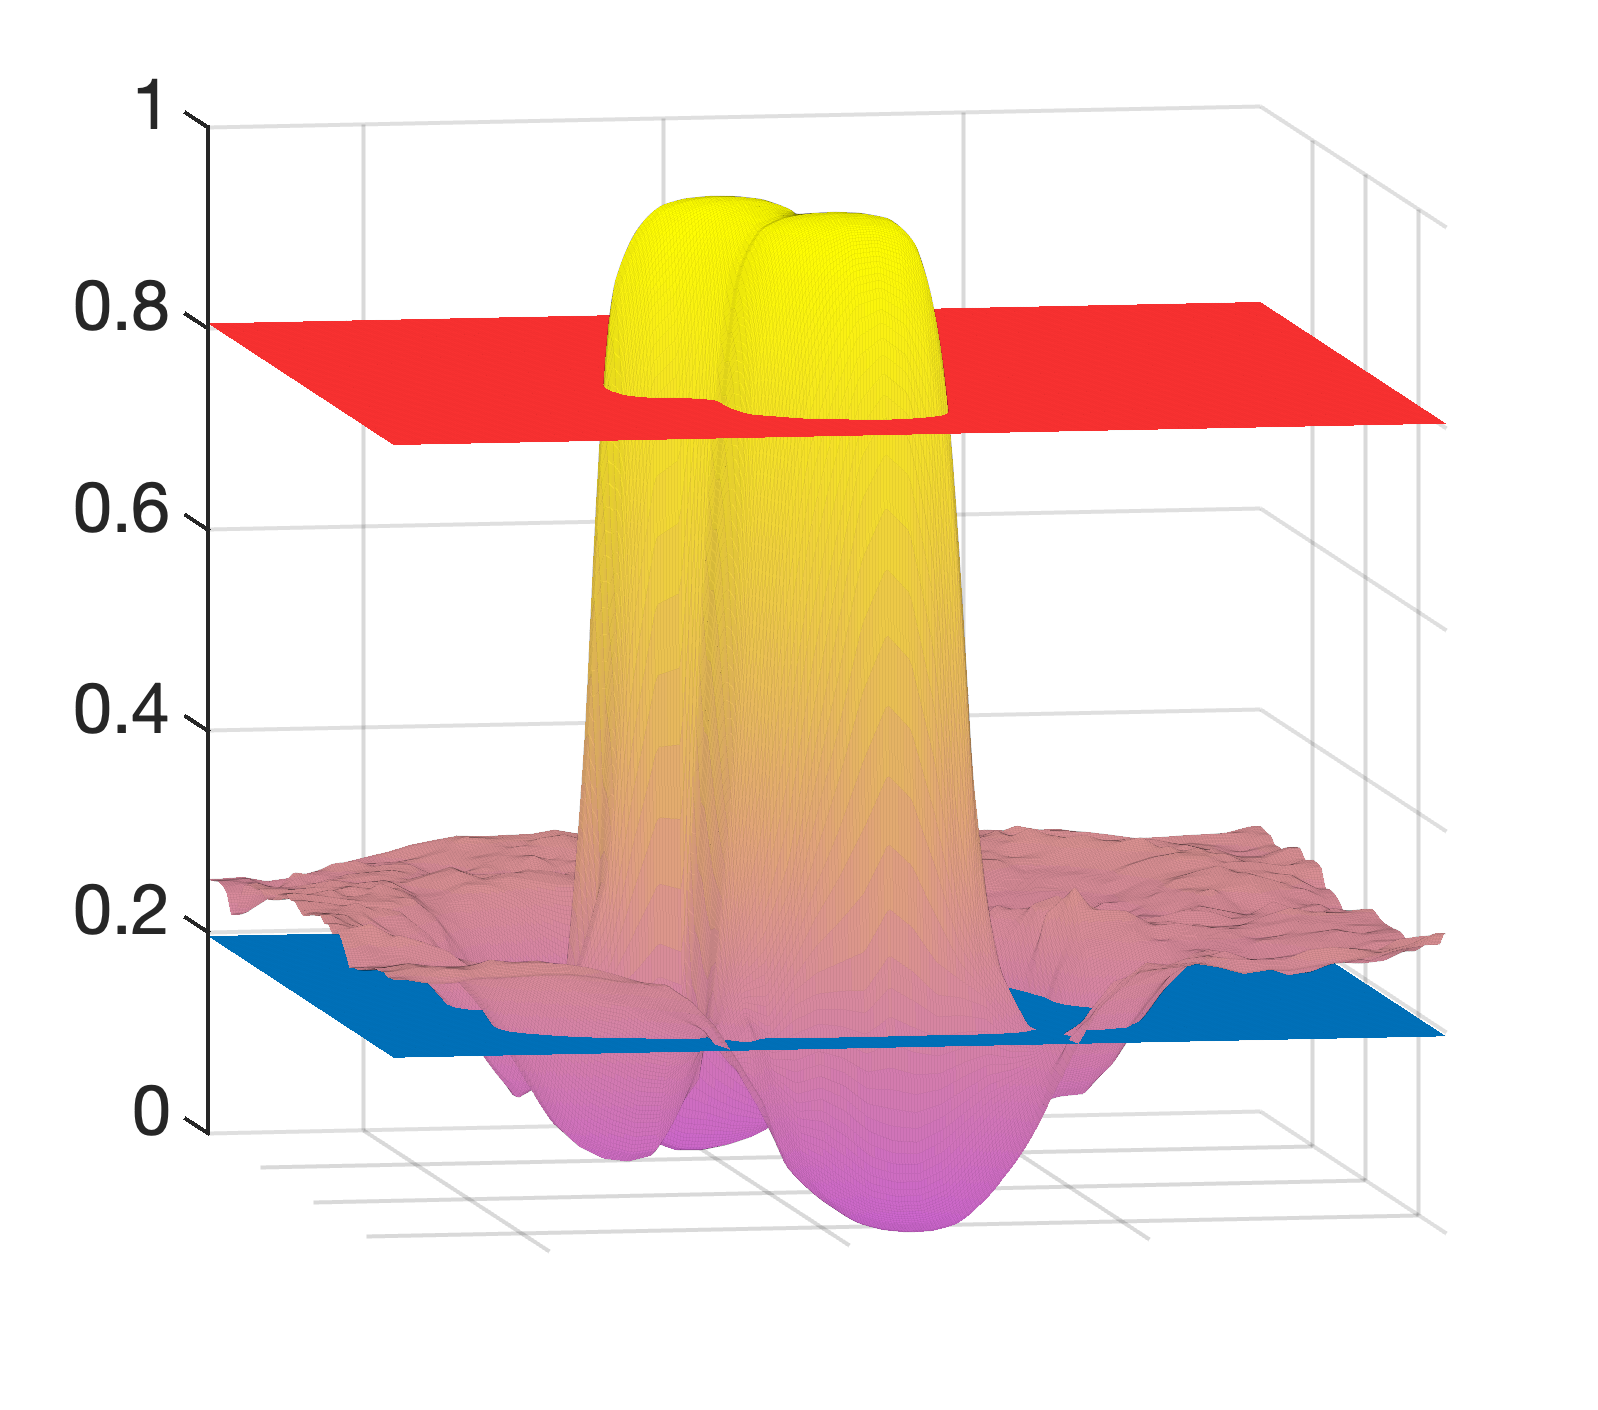
\includegraphics[width=0.24\textwidth]{../figures/learning/score_surf/754.png}	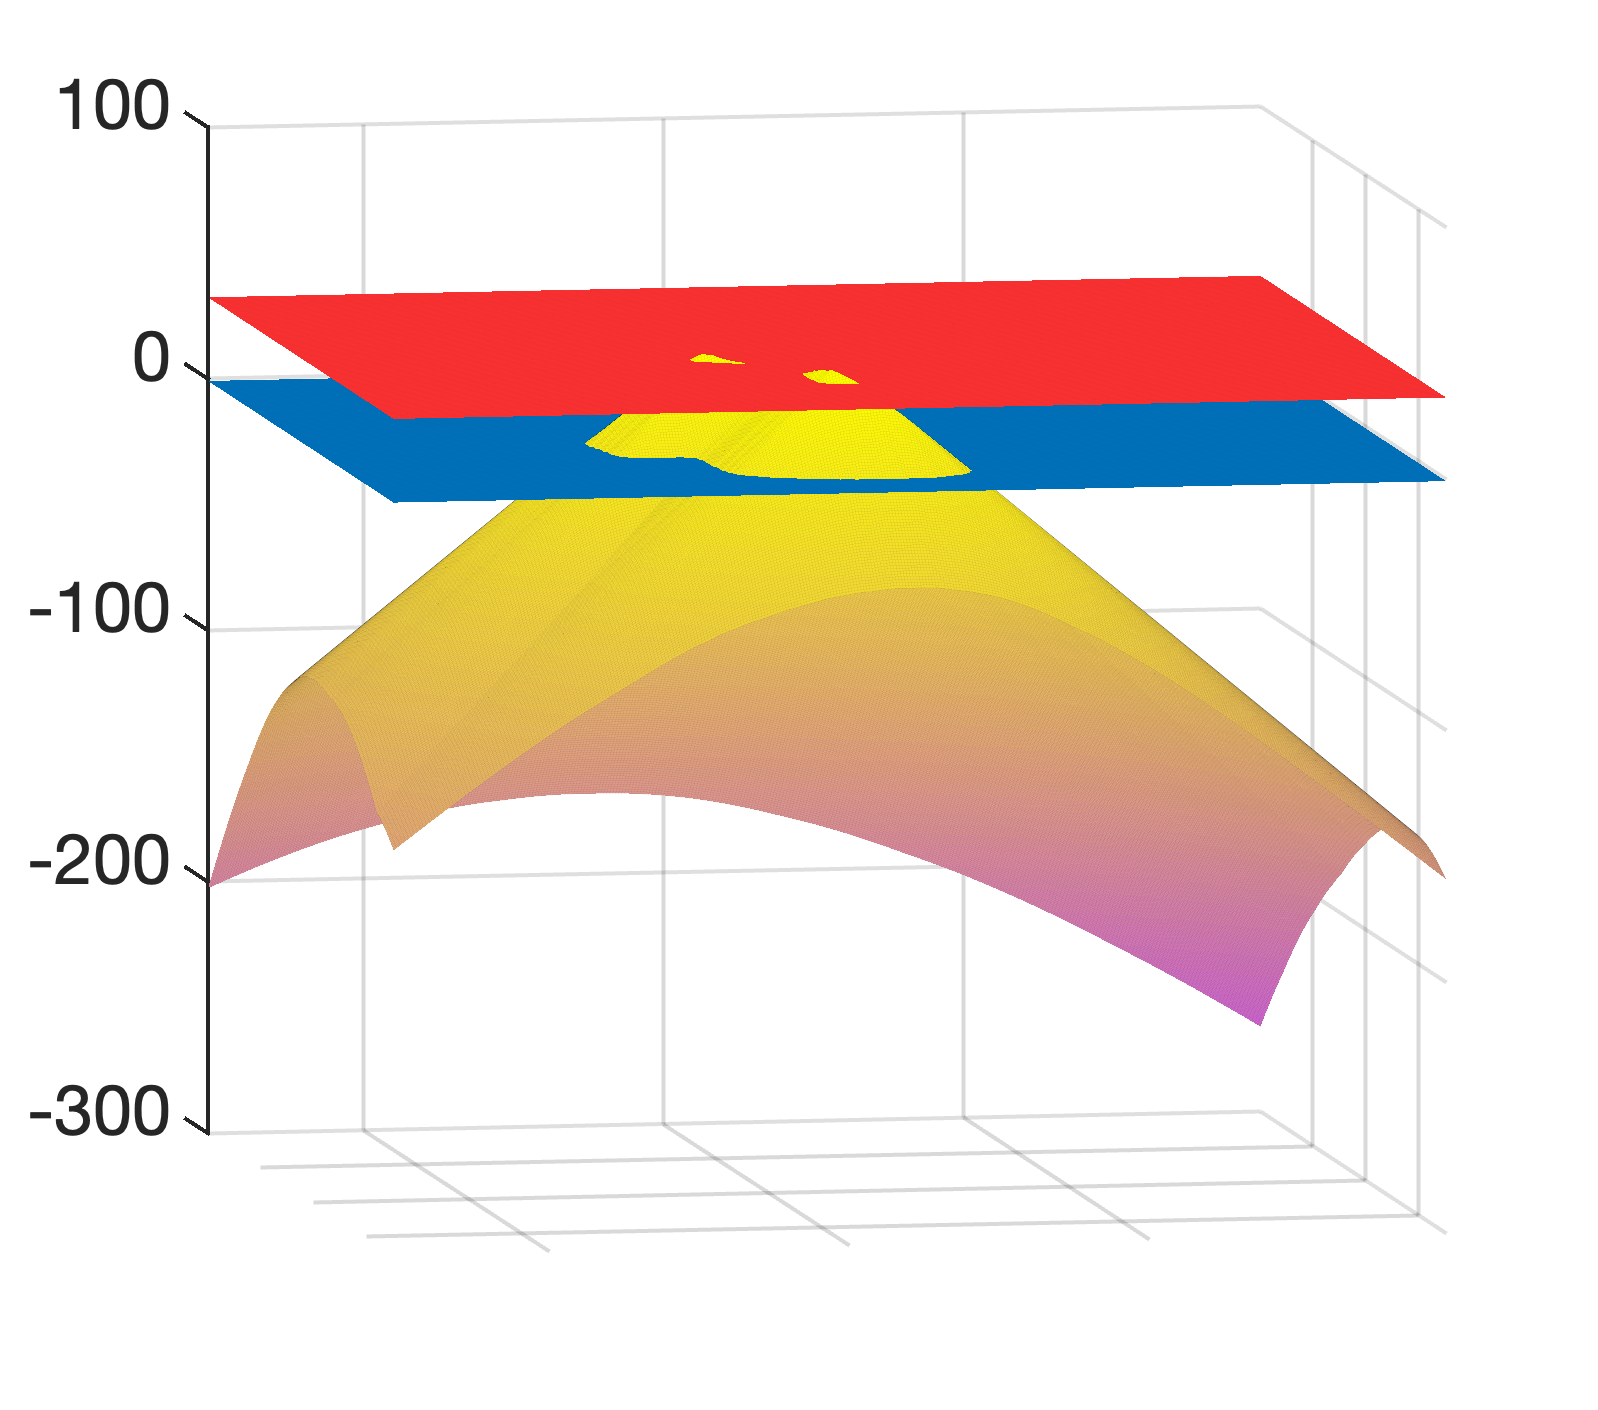
\includegraphics[width=0.24\textwidth]{../figures/learning/dist_surf/754.png}
		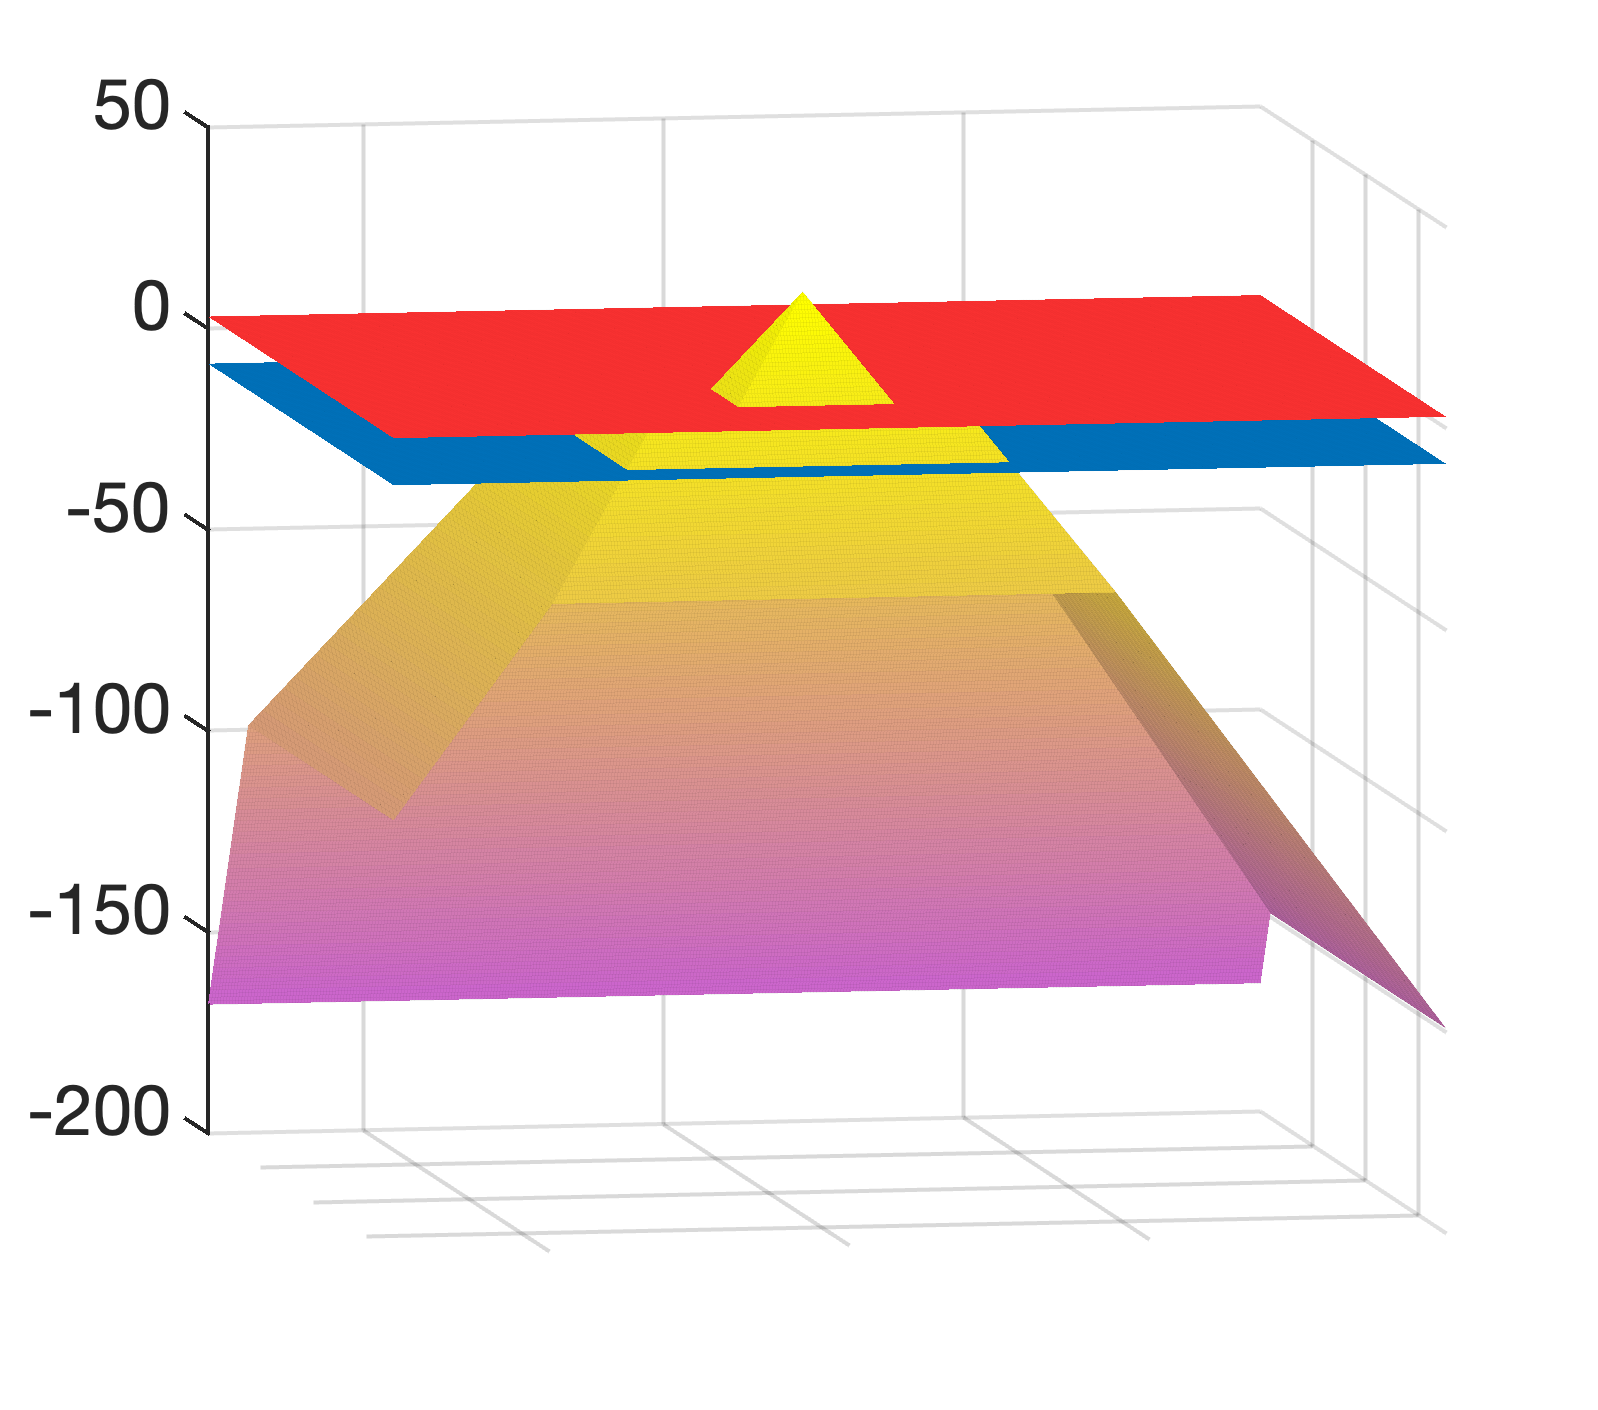
\includegraphics[width=0.24\textwidth]{../figures/learning/dist_bt_surf/754.png}\\
		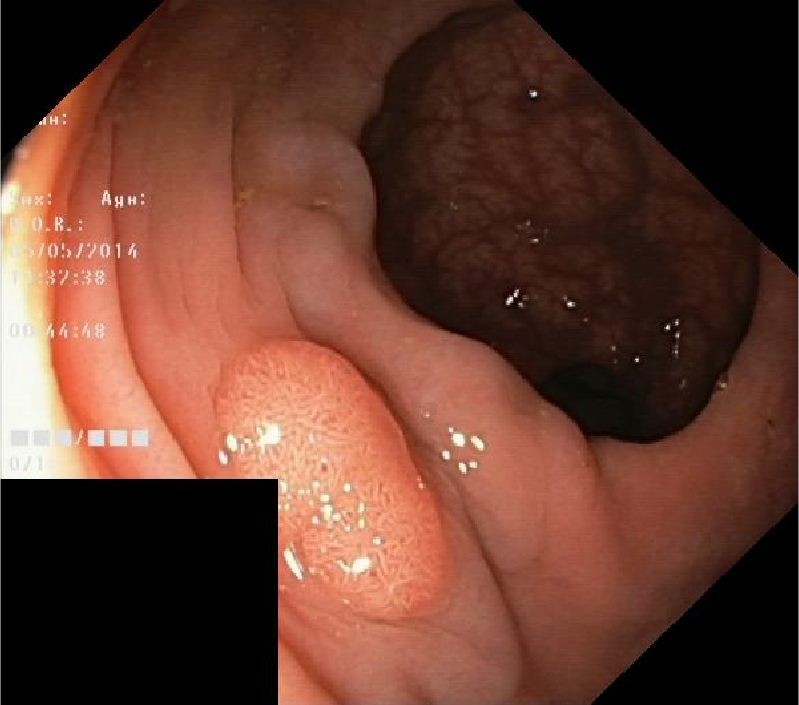
\includegraphics[width=0.24\textwidth]{../figures/learning/images/754.png}
		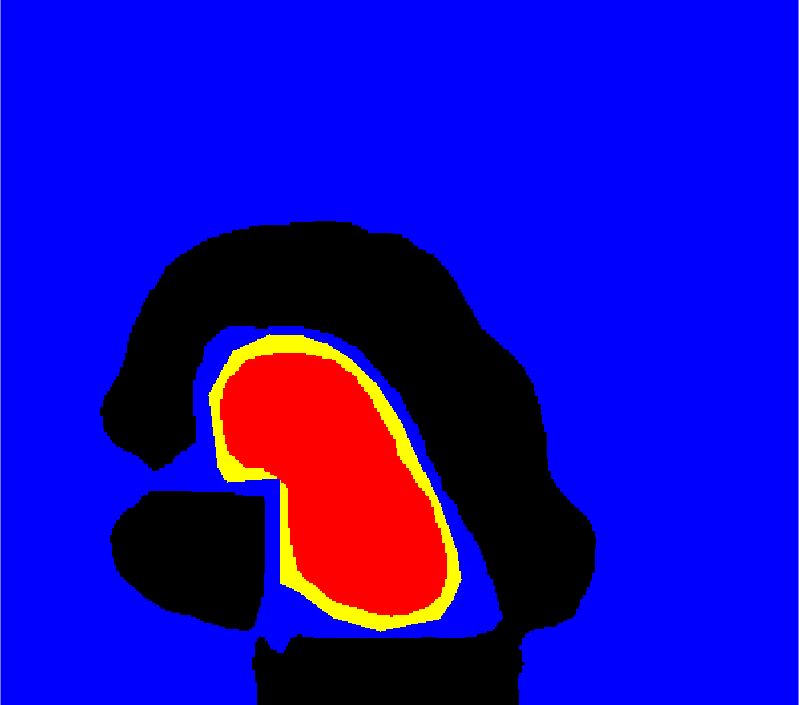
\includegraphics[width=0.24\textwidth]{../figures/learning/score_crs_marginal90/754.png}
		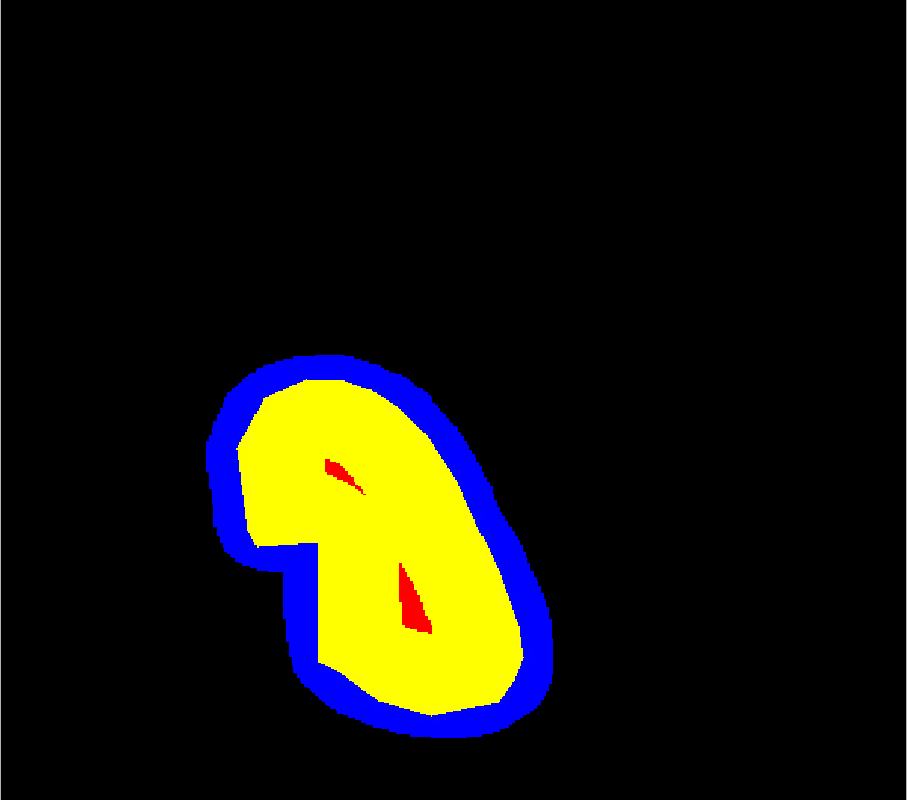
\includegraphics[width=0.24\textwidth]{../figures/learning/dist_crs_marginal90/754.png}
		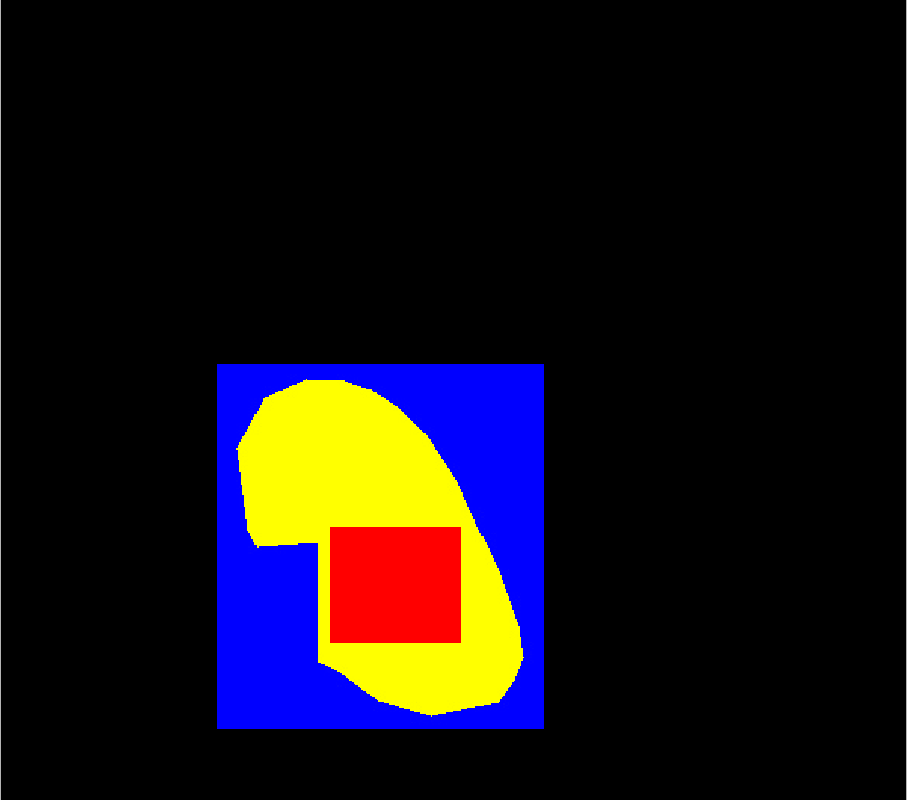
\includegraphics[width=0.24\textwidth]{../figures/learning/dist_bt_crs_marginal90/754.png}
	\end{center}
	\caption{Futher examples from the learning dataset. The layout of these figures is the same as for Figure \ref{fig:learning}.}
	\label{fig:learning3}
\end{figure}

\newpage
\subsection{Additional examples from the validation set}

